\documentclass{article}

% Hier befinden sich Pakete, die wir beinahe immer benutzen ...

\usepackage[utf8]{inputenc}

% Sprach-Paket:
\usepackage[ngerman]{babel}

% damit's nicht so, wie beim Grill aussieht:
\usepackage{fullpage}

% Mathematik:
\usepackage{amsmath, amssymb, amsfonts, amsthm}
\usepackage{bbm}
\usepackage{mathtools, mathdots}

% Makros mit mehereren Default-Argumenten:
\usepackage{twoopt}

% Anführungszeichen (Makro \Quote{}):
\usepackage{babel}

% if's für Makros:
\usepackage{xifthen}
\usepackage{etoolbox}

% tikz ist kein Zeichenprogramm (doch!):
\usepackage{tikz}

% bessere Aufzählungen:
\usepackage{enumitem}

% (bessere) Umgebung für Bilder:
\usepackage{graphicx, subfig, float}

% Umgebung für Code:
\usepackage{listings}

% Farben:
\usepackage{xcolor}

% Umgebung für "plain text":
\usepackage{verbatim}

% Umgebung für mehrerer Spalten:
\usepackage{multicol}

% "nette" Brüche
\usepackage{nicefrac}

% Spaltentypen verschiedener Dicke
\usepackage{tabularx}
\usepackage{makecell}

% Für Vektoren
\usepackage{esvect}

% (Web-)Links
\usepackage{hyperref}

% Zitieren & Literatur-Verzeichnis
\usepackage[style = authoryear]{biblatex}
\usepackage{csquotes}

% so ähnlich wie mathbb
%\usepackage{mathds}

% Keine Ahnung, was das macht ...
\usepackage{booktabs}
\usepackage{ngerman}
\usepackage{placeins}

% special letters:

\newcommand{\N}{\mathbb{N}}
\newcommand{\Z}{\mathbb{Z}}
\newcommand{\Q}{\mathbb{Q}}
\newcommand{\R}{\mathbb{R}}
\newcommand{\C}{\mathbb{C}}
\newcommand{\K}{\mathbb{K}}
\newcommand{\T}{\mathbb{T}}
\newcommand{\E}{\mathbb{E}}
\newcommand{\V}{\mathbb{V}}
\renewcommand{\S}{\mathbb{S}}
\renewcommand{\P}{\mathbb{P}}
\newcommand{\1}{\mathbbm{1}}

% quantors:

\newcommand{\Forall}{\forall \,}
\newcommand{\Exists}{\exists \,}
\newcommand{\ExistsOnlyOne}{\exists! \,}
\newcommand{\nExists}{\nexists \,}
\newcommand{\ForAlmostAll}{\forall^\infty \,}

% MISC symbols:

\newcommand{\landau}{{\scriptstyle \mathcal{O}}}
\newcommand{\Landau}{\mathcal{O}}


\newcommand{\eps}{\mathrm{eps}}

% graphics in a box:

\newcommandtwoopt
{\includegraphicsboxed}[3][][]
{
  \begin{figure}[!h]
    \begin{boxedin}
      \ifthenelse{\isempty{#1}}
      {
        \begin{center}
          \includegraphics[width = 0.75 \textwidth]{#3}
          \label{fig:#2}
        \end{center}
      }{
        \begin{center}
          \includegraphics[width = 0.75 \textwidth]{#3}
          \caption{#1}
          \label{fig:#2}
        \end{center}
      }
    \end{boxedin}
  \end{figure}
}

% braces:

\newcommand{\pbraces}[1]{{\left  ( #1 \right  )}}
\newcommand{\bbraces}[1]{{\left  [ #1 \right  ]}}
\newcommand{\Bbraces}[1]{{\left \{ #1 \right \}}}
\newcommand{\vbraces}[1]{{\left  | #1 \right  |}}
\newcommand{\Vbraces}[1]{{\left \| #1 \right \|}}
\newcommand{\abraces}[1]{{\left \langle #1 \right \rangle}}
\newcommand{\round}[1]{\bbraces{#1}}

\newcommand
{\floorbraces}[1]
{{\left \lfloor #1 \right \rfloor}}

\newcommand
{\ceilbraces} [1]
{{\left \lceil  #1 \right \rceil }}

% special functions:

\newcommand{\norm}  [2][]{\Vbraces{#2}_{#1}}
\newcommand{\diam}  [2][]{\mathrm{diam}_{#1} \: #2}
\newcommand{\diag}  [1]{\mathrm{diag} \: #1}
\newcommand{\dist}  [1]{\mathrm{dist} \: #1}
\newcommand{\mean}  [1]{\mathrm{mean} \: #1}
\newcommand{\erf}   [1]{\mathrm{erf} \: #1}
\newcommand{\id}    [1]{\mathrm{id} \: #1}
\newcommand{\sgn}   [1]{\mathrm{sgn} \: #1}
\newcommand{\supp}  [1]{\mathrm{supp} \: #1}
\newcommand{\arsinh}[1]{\mathrm{arsinh} \: #1}
\newcommand{\arcosh}[1]{\mathrm{arcosh} \: #1}
\newcommand{\artanh}[1]{\mathrm{artanh} \: #1}
\newcommand{\card}  [1]{\mathrm{card} \: #1}
\newcommand{\Span}  [1]{\mathrm{span} \: #1}
\newcommand{\Aut}   [1]{\mathrm{Aut} \: #1}
\newcommand{\End}   [1]{\mathrm{End} \: #1}
\newcommand{\ggT}   [1]{\mathrm{ggT} \: #1}
\newcommand{\kgV}   [1]{\mathrm{kgV} \: #1}
\newcommand{\ord}   [1]{\mathrm{ord} \: #1}
\newcommand{\grad}  [1]{\mathrm{grad} \: #1}
\newcommand{\ran}   [1]{\mathrm{ran} \: #1}
\newcommand{\graph} [1]{\mathrm{graph} \: #1}
\newcommand{\Inv}   [1]{\mathrm{Inv} \: #1}
\newcommand{\pv}    [1]{\mathrm{pv} \: #1}
\newcommand{\GL}    [1]{\mathrm{GL} \: #1}
\newcommand{\Mod}{\mathrm{Mod} \:}
\newcommand{\Th}{\mathrm{Th} \:}
\newcommand{\Char}{\mathrm{char}}
\newcommand{\At}{\mathrm{At}}
\newcommand{\Ob}{\mathrm{Ob}}
\newcommand{\Hom}{\mathrm{Hom}}
\newcommand{\orthogonal}[3][]{#2 ~\bot_{#1}~ #3}
\newcommand{\Rang}{\mathrm{Rang}}
\newcommand{\NIL}{\mathrm{NIL}}
\newcommand{\Res}{\mathrm{Res}}
\newcommand{\lxor}{\dot \lor}
\newcommand{\Div}{\mathrm{div} \:}
\newcommand{\meas}{\mathrm{meas} \:}

% fractions:

\newcommand{\Frac}[2]{\frac{1}{#1} \pbraces{#2}}
\newcommand{\nfrac}[2]{\nicefrac{#1}{#2}}

% derivatives & integrals:

\newcommandtwoopt
{\Int}[4][][]
{\int_{#1}^{#2} #3 ~\mathrm{d} #4}

\newcommandtwoopt
{\derivative}[3][][]
{
  \frac
  {\mathrm{d}^{#1} #2}
  {\mathrm{d} #3^{#1}}
}

\newcommandtwoopt
{\pderivative}[3][][]
{
  \frac
  {\partial^{#1} #2}
  {\partial #3^{#1}}
}

\newcommand
{\primeprime}
{{\prime \prime}}

\newcommand
{\primeprimeprime}
{{\prime \prime \prime}}

% Text:

\newcommand{\Quote}[1]{\glqq #1\grqq{}}
\newcommand{\Text}[1]{{\text{#1}}}
\newcommand{\fastueberall}{\text{f.ü.}}
\newcommand{\fastsicher}{\text{f.s.}}

% -------------------------------- %
% amsthm-stuff:

\theoremstyle{definition}

% numbered theorems
\newtheorem{theorem}{Satz}
\newtheorem{lemma}{Lemma}
\newtheorem{corollary}{Korollar}
\newtheorem{proposition}{Proposition}
\newtheorem{remark}{Bemerkung}
\newtheorem{definition}{Definition}
\newtheorem{example}{Beispiel}

% unnumbered theorems
\newtheorem*{theorem*}{Satz}
\newtheorem*{lemma*}{Lemma}
\newtheorem*{corollary*}{Korollar}
\newtheorem*{proposition*}{Proposition}
\newtheorem*{remark*}{Bemerkung}
\newtheorem*{definition*}{Definition}
\newtheorem*{example*}{Beispiel}

% Please define this stuff in project ("main.tex"):

% \def \lastexercisenumber {...}
% This will be 0 by default

% \setcounter{section}{...}
% This will be 0 by default
% and hence, completely ignored

\ifnum \thesection = 0
{\newtheorem{exercise}{Aufgabe}}
\else
{\newtheorem{exercise}{Aufgabe}[section]}
\fi

\ifdef
{\lastexercisenumber}
{\setcounter{exercise}{\lastexercisenumber}}

\newcommand{\solution}
{
    \renewcommand{\proofname}{Lösung}
    \renewcommand{\qedsymbol}{}
    \proof
}

\renewcommand{\proofname}{Beweis}

% -------------------------------- %
% environment zum einkasteln:

% dickere vertical lines
\newcolumntype
{x}
[1]
{!{\centering\arraybackslash\vrule width #1}}

% environment selbst (the big cheese)
\newenvironment
{boxedin}
{
  \begin{tabular}
  {
    x{1 pt}
    p{\textwidth}
    x{1 pt}
  }
  \Xhline
  {2 \arrayrulewidth}
}
{
  \\
  \Xhline{2 \arrayrulewidth}
  \end{tabular}
}

% -------------------------------- %
% MISC "Ein-Deutschungen"

\renewcommand
{\figurename}
{Abbildung}

\renewcommand
{\tablename}
{Tabelle}

% -------------------------------- %

% ---------------------------------------------------------------- %
% https://www.overleaf.com/learn/latex/Code_listing

\definecolor{codegreen} {rgb}{0, 0.6, 0}
\definecolor{codegray}    {rgb}{0.5, 0.5, 0.5}
\definecolor{codepurple}{rgb}{0.58, 0, 0.82}
\definecolor{backcolour}{rgb}{0.95, 0.95, 0.92}

\lstdefinestyle{overleaf}
{
    backgroundcolor = \color{backcolour},
    commentstyle = \color{codegreen},
    keywordstyle = \color{magenta},
    numberstyle = \tiny\color{codegray},
    stringstyle = \color{codepurple},
    basicstyle = \ttfamily \footnotesize,
    breakatwhitespace = false,
    breaklines = true,
    captionpos = b,
    keepspaces = true,
    numbers = left,
    numbersep = 5pt,
    showspaces = false,
    showstringspaces = false,
    showtabs = false,
    tabsize = 2
}

% ---------------------------------------------------------------- %
% https://en.wikibooks.org/wiki/LaTeX/Source_Code_Listings

\lstdefinestyle{customc}
{
    belowcaptionskip = 1 \baselineskip,
    breaklines = true,
    frame = L,
    xleftmargin = \parindent,
    language = C,
    showstringspaces = false,
    basicstyle = \footnotesize \ttfamily,
    keywordstyle = \bfseries \color{green!40!black},
    commentstyle = \itshape \color{purple!40!black},
    identifierstyle = \color{blue},
    stringstyle = \color{orange},
}

\lstdefinestyle{customasm}
{
    belowcaptionskip = 1 \baselineskip,
    frame = L,
    xleftmargin = \parindent,
    language = [x86masm] Assembler,
    basicstyle = \footnotesize\ttfamily,
    commentstyle = \itshape\color{purple!40!black},
}

% ---------------------------------------------------------------- %
% https://tex.stackexchange.com/questions/235731/listings-syntax-for-literate

\definecolor{maroon}        {cmyk}{0, 0.87, 0.68, 0.32}
\definecolor{halfgray}      {gray}{0.55}
\definecolor{ipython_frame} {RGB}{207, 207, 207}
\definecolor{ipython_bg}    {RGB}{247, 247, 247}
\definecolor{ipython_red}   {RGB}{186, 33, 33}
\definecolor{ipython_green} {RGB}{0, 128, 0}
\definecolor{ipython_cyan}  {RGB}{64, 128, 128}
\definecolor{ipython_purple}{RGB}{170, 34, 255}

\lstdefinestyle{stackexchangePython}
{
    breaklines = true,
    %
    extendedchars = true,
    literate =
    {á}{{\' a}} 1 {é}{{\' e}} 1 {í}{{\' i}} 1 {ó}{{\' o}} 1 {ú}{{\' u}} 1
    {Á}{{\' A}} 1 {É}{{\' E}} 1 {Í}{{\' I}} 1 {Ó}{{\' O}} 1 {Ú}{{\' U}} 1
    {à}{{\` a}} 1 {è}{{\` e}} 1 {ì}{{\` i}} 1 {ò}{{\` o}} 1 {ù}{{\` u}} 1
    {À}{{\` A}} 1 {È}{{\' E}} 1 {Ì}{{\` I}} 1 {Ò}{{\` O}} 1 {Ù}{{\` U}} 1
    {ä}{{\" a}} 1 {ë}{{\" e}} 1 {ï}{{\" i}} 1 {ö}{{\" o}} 1 {ü}{{\" u}} 1
    {Ä}{{\" A}} 1 {Ë}{{\" E}} 1 {Ï}{{\" I}} 1 {Ö}{{\" O}} 1 {Ü}{{\" U}} 1
    {â}{{\^ a}} 1 {ê}{{\^ e}} 1 {î}{{\^ i}} 1 {ô}{{\^ o}} 1 {û}{{\^ u}} 1
    {Â}{{\^ A}} 1 {Ê}{{\^ E}} 1 {Î}{{\^ I}} 1 {Ô}{{\^ O}} 1 {Û}{{\^ U}} 1
    {œ}{{\oe}}  1 {Œ}{{\OE}}  1 {æ}{{\ae}}  1 {Æ}{{\AE}}  1 {ß}{{\ss}}  1
    {ç}{{\c c}} 1 {Ç}{{\c C}} 1 {ø}{{\o}} 1 {å}{{\r a}} 1 {Å}{{\r A}} 1
    {€}{{\EUR}} 1 {£}{{\pounds}} 1
}


% Python definition (c) 1998 Michael Weber
% Additional definitions (2013) Alexis Dimitriadis
% modified by me (should not have empty lines)

\lstdefinelanguage{iPython}{
    morekeywords = {access, and, break, class, continue, def, del, elif, else, except, exec, finally, for, from, global, if, import, in, is, lambda, not, or, pass, print, raise, return, try, while}, %
    %
    % Built-ins
    morekeywords = [2]{abs, all, any, basestring, bin, bool, bytearray, callable, chr, classmethod, cmp, compile, complex, delattr, dict, dir, divmod, enumerate, eval, execfile, file, filter, float, format, frozenset, getattr, globals, hasattr, hash, help, hex, id, input, int, isinstance, issubclass, iter, len, list, locals, long, map, max, memoryview, min, next, object, oct, open, ord, pow, property, range, raw_input, reduce, reload, repr, reversed, round, set, setattr, slice, sorted, staticmethod, str, sum, super, tuple, type, unichr, unicode, vars, xrange, zip, apply, buffer, coerce, intern}, %
    %
    sensitive = true, %
    morecomment = [l] \#, %
    morestring = [b]', %
    morestring = [b]", %
    %
    morestring = [s]{'''}{'''}, % used for documentation text (mulitiline strings)
    morestring = [s]{"""}{"""}, % added by Philipp Matthias Hahn
    %
    morestring = [s]{r'}{'},     % `raw' strings
    morestring = [s]{r"}{"},     %
    morestring = [s]{r'''}{'''}, %
    morestring = [s]{r"""}{"""}, %
    morestring = [s]{u'}{'},     % unicode strings
    morestring = [s]{u"}{"},     %
    morestring = [s]{u'''}{'''}, %
    morestring = [s]{u"""}{"""}, %
    %
    % {replace}{replacement}{lenght of replace}
    % *{-}{-}{1} will not replace in comments and so on
    literate = 
    {á}{{\' a}} 1 {é}{{\' e}} 1 {í}{{\' i}} 1 {ó}{{\' o}} 1 {ú}{{\' u}} 1
    {Á}{{\' A}} 1 {É}{{\' E}} 1 {Í}{{\' I}} 1 {Ó}{{\' O}} 1 {Ú}{{\' U}} 1
    {à}{{\` a}} 1 {è}{{\` e}} 1 {ì}{{\` i}} 1 {ò}{{\` o}} 1 {ù}{{\` u}} 1
    {À}{{\` A}} 1 {È}{{\' E}} 1 {Ì}{{\` I}} 1 {Ò}{{\` O}} 1 {Ù}{{\` U}} 1
    {ä}{{\" a}} 1 {ë}{{\" e}} 1 {ï}{{\" i}} 1 {ö}{{\" o}} 1 {ü}{{\" u}} 1
    {Ä}{{\" A}} 1 {Ë}{{\" E}} 1 {Ï}{{\" I}} 1 {Ö}{{\" O}} 1 {Ü}{{\" U}} 1
    {â}{{\^ a}} 1 {ê}{{\^ e}} 1 {î}{{\^ i}} 1 {ô}{{\^ o}} 1 {û}{{\^ u}} 1
    {Â}{{\^ A}} 1 {Ê}{{\^ E}} 1 {Î}{{\^ I}} 1 {Ô}{{\^ O}} 1 {Û}{{\^ U}} 1
    {œ}{{\oe}}  1 {Œ}{{\OE}}  1 {æ}{{\ae}}  1 {Æ}{{\AE}}  1 {ß}{{\ss}}  1
    {ç}{{\c c}} 1 {Ç}{{\c C}} 1 {ø}{{\o}} 1 {å}{{\r a}} 1 {Å}{{\r A}} 1
    {€}{{\EUR}} 1 {£}{{\pounds}} 1
    %
    {^}{{{\color{ipython_purple}\^ {}}}} 1
    { = }{{{\color{ipython_purple} = }}} 1
    %
    {+}{{{\color{ipython_purple}+}}} 1
    {*}{{{\color{ipython_purple}$^\ast$}}} 1
    {/}{{{\color{ipython_purple}/}}} 1
    %
    {+=}{{{+=}}} 1
    {-=}{{{-=}}} 1
    {*=}{{{$^\ast$ = }}} 1
    {/=}{{{/=}}} 1,
    literate = 
    *{-}{{{\color{ipython_purple} -}}} 1
     {?}{{{\color{ipython_purple} ?}}} 1,
    %
    identifierstyle = \color{black}\ttfamily,
    commentstyle = \color{ipython_cyan}\ttfamily,
    stringstyle = \color{ipython_red}\ttfamily,
    keepspaces = true,
    showspaces = false,
    showstringspaces = false,
    %
    rulecolor = \color{ipython_frame},
    frame = single,
    frameround = {t}{t}{t}{t},
    framexleftmargin = 6mm,
    numbers = left,
    numberstyle = \tiny\color{halfgray},
    %
    %
    backgroundcolor = \color{ipython_bg},
    % extendedchars = true,
    basicstyle = \scriptsize,
    keywordstyle = \color{ipython_green}\ttfamily,
}

% ---------------------------------------------------------------- %
% https://tex.stackexchange.com/questions/417884/colour-r-code-to-match-knitr-theme-using-listings-minted-or-other

\geometry{verbose, tmargin = 2.5cm, bmargin = 2.5cm, lmargin = 2.5cm, rmargin = 2.5cm}

\definecolor{backgroundCol}  {rgb}{.97, .97, .97}
\definecolor{commentstyleCol}{rgb}{0.678, 0.584, 0.686}
\definecolor{keywordstyleCol}{rgb}{0.737, 0.353, 0.396}
\definecolor{stringstyleCol} {rgb}{0.192, 0.494, 0.8}
\definecolor{NumCol}         {rgb}{0.686, 0.059, 0.569}
\definecolor{basicstyleCol}  {rgb}{0.345, 0.345, 0.345}

\lstdefinestyle{stackexchangeR}
{
    language = R,                                        % the language of the code
    basicstyle = \small \ttfamily \color{basicstyleCol}, % the size of the fonts that are used for the code
    % numbers = left,                                      % where to put the line-numbers
    numberstyle = \color{green},                         % the style that is used for the line-numbers
    stepnumber = 1,                                      % the step between two line-numbers. If it is 1, each line will be numbered
    numbersep = 5pt,                                     % how far the line-numbers are from the code
    backgroundcolor = \color{backgroundCol},             % choose the background color. You must add \usepackage{color}
    showspaces = false,                                  % show spaces adding particular underscores
    showstringspaces = false,                            % underline spaces within strings
    showtabs = false,                                    % show tabs within strings adding particular underscores
    % frame = single,                                      % adds a frame around the code
    % rulecolor = \color{white},                           % if not set, the frame-color may be changed on line-breaks within not-black text (e.g. commens (green here))
    tabsize = 2,                                         % sets default tabsize to 2 spaces
    captionpos = b,                                      % sets the caption-position to bottom
    breaklines = true,                                   % sets automatic line breaking
    breakatwhitespace = false,                           % sets if automatic breaks should only happen at whitespace
    keywordstyle = \color{keywordstyleCol},              % keyword style
    commentstyle = \color{commentstyleCol},              % comment style
    stringstyle = \color{stringstyleCol},                % string literal style
    literate = %
    *{0}{{{\color{NumCol} 0}}} 1
     {1}{{{\color{NumCol} 1}}} 1
     {2}{{{\color{NumCol} 2}}} 1
     {3}{{{\color{NumCol} 3}}} 1
     {4}{{{\color{NumCol} 4}}} 1
     {5}{{{\color{NumCol} 5}}} 1
     {6}{{{\color{NumCol} 6}}} 1
     {7}{{{\color{NumCol} 7}}} 1
     {8}{{{\color{NumCol} 8}}} 1
     {9}{{{\color{NumCol} 9}}} 1
}

% ---------------------------------------------------------------- %
% Fundament Mathematik

\lstdefinestyle{fundament}{basicstyle = \ttfamily}

% ---------------------------------------------------------------- %


\parskip 0pt
\parindent 0pt

\title
{
  Maß- und Wahrscheinlichkeitstheorie 1 \\
  \vspace{4pt}
  \normalsize
  \textit{Prüfungsbeispiele}
}

\author
{Richard Weiss}

\date{}

\begin{document}

\maketitle

\section{Menensysteme und Maßfunktionen}

\begin{exercise}

Hier könnte Ihre Werbung stehen!

\begin{itemize}
  \item[(a)] Definieren Sie Maßfunktion, endliche Maßfunktion, sigmaendliche Maßfunktion, äußere Maßfunktion.
  \item[(b)] Formulieren und beweisen Sie den Fortsetzungssatz für Maßfunktionen.
  \item[(c)] $\Omega$ sei eine beliebige Menge für $A \subseteq \Omega$
  \begin{align*}
    \mu^\ast(A) =
    \begin{cases}
      0, & \text{wenn} \enspace A = \emptyset, \\
      1, & \text{sonst}.
    \end{cases}
  \end{align*}
  Zeigen Sie, dass $\mu^\ast$ eine äußere Maßfunktion ist und bestimmen Sie das System der $\mu^\ast$-messbaren Mengen.
\end{itemize}

\end{exercise}

\begin{solution}

Sei $\mu: \mathfrak{C} \to \R$ eine Mengenfunktion auf dem Mengensystem $\emptyset \neq \mathfrak{C} \subseteq 2^\Omega$.

\begin{itemize}

  \item $\mu \Text{Maßfunktion} : \Leftrightarrow$
  \begin{itemize}
    \item $\Forall A \in \mathfrak{C}: \mu(A) \geq 0,$
    \item $\mu \enspace \sigma \text{-additiv}, \enspace
    \text{d.h.}
    \Forall (A_n) \in \mathfrak{C}, \text{disj.}, \text{höchst. abz.}:
    A := \sum_{n \in \N} A_n \in \mathfrak{C} \Rightarrow
    \mu(A) = \sum_{n \in \N} \mu(A_n)$
  \end{itemize}

  \item $\mu \Text{endliche Maßfunktion} : \Leftrightarrow$
  \begin{itemize}
    \item $\mu \enspace \text{Maßfunktion},$
    \item $\Forall A \in \mathfrak{C}: \mu(A) < \infty$
  \end{itemize}

  \item $\mu \Text{sigmaendliche Maßfunktion} : \Leftrightarrow$
  \begin{itemize}
    \item $\mu \enspace \text{Maßfunktion},$
    \item $\Forall A \in \mathfrak{C}: \Exists (A_n) \in \mathfrak{C}: A \subseteq \bigcup_{n \in \N} A_n, \Forall n \in \N: \mu(A_n) < \infty$
  \end{itemize}

\end{itemize}

Sei $\mu^\ast: 2^\Omega \to \R$ eine weitere Mengenfunktion.

\begin{itemize}

  \item $\mu^\ast \Text{äußere Maßfunktion} : \Leftrightarrow$
  \begin{itemize}
    \item $\mu^\ast(\emptyset) = 0,$
    \item $\Forall A \in 2^\Omega: \mu^\ast(A) \geq 0,$
    \item $\Forall A, B \in 2^\Omega:
    A \subseteq B \Rightarrow
    \mu^\ast(A) \leq \mu^\ast(B),$
    \item $\Forall A, (B_n) \in 2^\Omega:
    A \subseteq \bigcup_{n \in \N} B_n \Rightarrow
    \mu^\ast(A) \leq \sum_{n \in \N} \mu^\ast(B_n)$
  \end{itemize}

\end{itemize}

Der Beweis des Fortsetzungssatz für Maßfunktionen ist nicht teil des Prüfungsstoffs. Dennoch, er besagt folgendes.

\begin{theorem*}[Fortsetzungssatz für Maßfunktionen]

$\mu$ sei ein Maß auf einem Semiring $\mathfrak{T}$. Dann kann man auf dem von $\mathfrak{T}$ erzeugten Sigmaring ein Maß finden, dass auf $\mathfrak{T}$ mit $\mu$ übereinstimmt. \\
Wenn $\mu$ auf $\mathfrak{T}$ sigmaendlich ist, dann ist die Fortsetzung auf den erzeugten Sigmaring eindeutig bestimmt.

\end{theorem*}

Die ersten drei Eigenschaften sind offensichtlich. Seien zuletzt $A, (B_n) \in 2^\Omega$ mit $A \subseteq \bigcup_{n \in \N} B_n$. Falls $A = \emptyset$, sind wir (wegen der zweiten Eigenschaft) fertig und sonst $\Exists n \in \N: B_n \neq \emptyset$. \\

Das System der Carathéodory-messbaren Mengen lautet wie folgt.

\begin{align*}
  \mathfrak{M}_{\mu^\ast} :=
  \Bbraces
  {
    A \subseteq \Omega:
    \Forall B \subseteq \Omega:
    \mu^\ast(B) = \mu^\ast(B \cap A) + \mu^\ast(B \cap A^\complement)
  }
\end{align*}

Weil dieses System eine $\sigma$-Algebra ist, sind $\emptyset, \Omega$ messbar. $A \subseteq \Omega$ mit $A \neq \emptyset, \Omega$, ist wegen $B := \Omega$ nicht messbar, weil $A^\complement \neq \emptyset$ und damit $\mathfrak{M}_{\mu^\ast} = \Bbraces{\emptyset, \Omega}$.

\end{solution}

--------------------------------------------------------------------------------

\begin{exercise}

Gegeben sei die folgende Funktion auf $2^\R$:

\begin{align*}
  \mu^\ast(A) =
  \begin{cases}
    0 & \text{für} \enspace A = \emptyset, \\
    1 & \text{wenn} \enspace 1 \leq |A| < \infty, \\
    2 & \text{sonst}.
  \end{cases}
\end{align*}

Zeigen Sie, dass $\mu^\ast$ eine äußere Maßfunktion ist und bestimmen Sie das System der $\mu^\ast$-messbaren Mengen.

\end{exercise}

\begin{solution}

Die ersten drei Eigenschaften sind offensichtlich. Seien zuletzt $A, (B_n) \in 2^\Omega$ mit $A \subseteq \bigcup_{n \in \N} B_n$. Falls $A = \emptyset$, sind wir (wegen der zweiten Eigenschaft) fertig. Für $1 \leq |A| < \infty$, muss $\Exists n \in \N: 1 \leq |B_n| < \infty$. Ansonsten, sind die (unendlich vielen) $\omega \in A$ über ganz $(B_n)$ verteilt. Nun gilt aber $\Exists n \in \N: |B_n| = \infty$ oder $\Exists n \neq m \in \N: 1 \leq |B_n|, |B_m| < \infty$. \\

Das System der Carathéodory-messbaren Mengen lautet wie folgt.

\begin{align*}
  \mathfrak{M}_{\mu^\ast} :=
  \Bbraces
  {
    A \subseteq \Omega:
    \Forall B \subseteq \Omega:
    \mu^\ast(B) = \mu^\ast(B \cap A) + \mu^\ast(B \cap A^\complement)
  }
\end{align*}

Weil dieses System eine $\sigma$-Algebra ist, sind $\emptyset, \Omega$ messbar. Sei also $A \subseteq \Omega$ mit $A \neq \emptyset, \Omega$.

\begin{itemize}

  \item[Fall $1$)] $A \enspace \text{endl.} \Rightarrow A^\complement \Text{unendl.}$
  \begin{align*}
    2 = \mu^\ast(\R) =
    \underbrace{\mu^\ast(\R \cap A)}_1 +
    \underbrace{\mu^\ast(\R \cap A^\complement)}_2 = 3
  \end{align*}

  \item[Fall $2$)] $A \enspace \text{unendl.}$
  \begin{itemize}
    \item[Fall a)] $A^\complement \enspace \text{endl.} \Rightarrow$ analog zu Fall $1$
    \item[Fall b)] $A^\complement \enspace \text{unendl.}$
    \begin{align*}
      2 = \mu^\ast(\R) =
      \underbrace{\mu^\ast(\R \cap A)}_2 +
      \underbrace{\mu^\ast(\R \cap A^\complement)}_2 = 4
    \end{align*}
  \end{itemize}

\end{itemize}

Damit, muss $\mathfrak{M}_{\mu^\ast} = \Bbraces{\emptyset, \Omega}$.

\end{solution}

--------------------------------------------------------------------------------

\begin{exercise}

Hier könnte Ihre Werbung stehen!

\begin{itemize}
  \item[(a)] Definieren Sie Ring, Semiring, monotones System, Dynkin-System, Algebra, Sigmaalgebra.
  \item[(b)] Zeigen Sie: Wenn $\mathfrak{R}$ ein Ring ist, dann stimmt das von $\mathfrak{R}$ erzeugte monotone System mit dem erzeugten Sigmaring überein.
\end{itemize}

\end{exercise}

\begin{solution}

Hier könnte Ihre Werbung stehen!

\begin{itemize}

  \item $\emptyset \neq \mathfrak{R} \subseteq 2^\Omega \Text{Ring} : \Leftrightarrow \Forall A, B \in \mathfrak{R}:$
  \begin{itemize}
    \item $A \cup B \in \mathfrak{R}$
    \item $A \setminus B \in \mathfrak{R}$
  \end{itemize}

  \item $\emptyset \neq \mathfrak{T} \subseteq 2^\Omega \Text{Semiring} : \Leftrightarrow \Forall A, B \in \mathfrak{T}:$
  \begin{itemize}
    \item $A \cap B \in \mathfrak{T},$
    \item $A \subseteq B \Rightarrow \Exists C_1, \ldots, C_n \in \mathfrak{T}, \Text{disj.}:
    B \setminus A = \sum_{i=1}^n C_i,$
    \item $\Forall k = 1, \ldots, n:
    A \cup \sum_{i=1}^k C_i \in \mathfrak{T}$
  \end{itemize}

  \item $\mathfrak{M} \subseteq 2^\Omega \Text{monotones System} : \Leftrightarrow \Forall (A_n) \in \mathfrak{M}, \Text{mon.}: \lim_{n \to \infty} A_n \in \mathfrak{M}$

  \item $\emptyset \neq \mathfrak{D} \subseteq 2^\Omega \Text{Dynkin-System} : \Leftrightarrow$
  \begin{itemize}
    \item $\Forall A, B \in \mathfrak{D}:
    A \subseteq B \Rightarrow B \setminus A \in \mathfrak{D}$
    \item $\Forall (A_n) \in \mathfrak{D}, \text{disj.}: \sum_{n \in \N} A_n \in \mathfrak{D}$
    \item $\Omega \in \mathfrak{D}$
  \end{itemize}

  \item $\emptyset \neq \mathfrak{A} \subseteq 2^\Omega \Text{Algebra} : \Leftrightarrow$
  \begin{itemize}
    \item $\mathfrak{A} \enspace \text{Ring},$
    \item $\Omega \in \mathfrak{A}$
  \end{itemize}

  \item $\emptyset \neq \mathfrak{A}_\sigma \subseteq 2^\Omega \Text{Sigmaalgebra} : \Leftrightarrow$
  \begin{itemize}
    \item $\Forall (A_n) \in \mathfrak{A}_\sigma, \text{disj.}: \sum_{n \in \N} A_n \in \mathfrak{A}_\sigma$
    \item $\Forall A, B \in \mathfrak{A}_\sigma: A \setminus B \in \mathfrak{A}_\sigma,$
    \item $\Omega \in \mathfrak{A}_\sigma$
  \end{itemize}

\end{itemize}

Der nächste Teil ist genau das \Quote{Monotone Class Theorem} und steht woanders!

\end{solution}

--------------------------------------------------------------------------------

\begin{exercise}

Hier könnte Ihre Werbung stehen!

\begin{itemize}
  \item[(a)] Definieren sie Maßfunktion, endliche Maßfunktion, sigmaendliche Maßfunktion, äußere Maßfunktion, von einem Maß erzeugte äußere Maßfunktion.
  \item[(b)] Zeigen Sie, dass eine äußere Maßfunktion auf dem System der messbaren Mengen ein Maß bildet.
\end{itemize}

\end{exercise}

\begin{solution}

(a) Sei $\inf \emptyset := \infty$. Dann ist die äußere Maßfunktion, für ein Maß $\mu$ auf einem Ring $\mathfrak{R}$, definiert als

\begin{align*}
  \mu^\ast:
  2^\Omega \to \bar \R,
  A \mapsto \inf \Bbraces{\sum_{n \in \N} \mu(E_n): (E_n) \in \mathfrak{R}, A \subseteq \bigcup_{n \in \N} E_n}.
\end{align*}

Für den Rest: siehe Aufgabe 1 (a). \\

(b) Siehe Skript.

\end{solution}

--------------------------------------------------------------------------------

\begin{exercise}

Hier könnte Ihre Werbung stehen!

\begin{itemize}
  \item[(a)] $\mathfrak{S}$ sei eine Sigmaalgebra über $\Omega$, $\mathfrak{C} \subset \Omega$. Zeigen Sie
  \begin{align*}
    \mathfrak{A}_\sigma(\mathfrak{S} \cup \Bbraces{C}) =
    \Bbraces{(A \cap C) \cup (B \cap C^\complement), A, B \in \mathfrak{S}}.
  \end{align*}
  \item[(b)] $\mathfrak{R}$ sei ein Ring über $\Omega$. Zeigen Sie
  \begin{align*}
    \mathfrak{A}(\mathfrak{R}) =
    \mathfrak{R} \cup \Bbraces{A: A^\complement \in \mathfrak{R}}.
  \end{align*}
\end{itemize}

\end{exercise}

\begin{solution}

(a) \Quote{$\supseteq$}: Seien $A, B \in \mathfrak{S}$, dann auch $A, B, C \in \mathfrak{A}_\sigma(\mathfrak{S} \cup \Bbraces{C})$. Als $\sigma$-Algebra ist diese bezüglich \Quote{$\cap$}, \Quote{$\cup$}, \Quote{$^\complement$} abgeschlossen. \\

\Quote{$\subseteq$}: Die linke Seite ist die kleinste $\sigma$-Algebra, die $\mathfrak{S} \cup \Bbraces{C}$ enthält. Sei $\mathfrak{S}^\prime$ die rechte Seite, dann muss

\begin{itemize}
  \item $\mathfrak{S} \subseteq \mathfrak{S}^\prime$, wenn man $A = B$ wählt und
  \item $C \in \mathfrak{S}^\prime$, wenn $A := \Omega$, $B := \emptyset$.
\end{itemize}

Wir weisen also noch nach, dass $\mathfrak{S}^\prime$ eine $\sigma$-Algebra ist.

\begin{itemize}

  \item \Quote{Enthält Grundmenge}: $\Omega \in \mathfrak{S} \subseteq \mathfrak{S}^\prime$

  \item \Quote{Stabil bzgl. abzählbaren Vereinigungen}: Sei $(E_n) \in \mathfrak{S}^\prime$, dann $\Exists (A_n), (B_n) \in \mathfrak{S}:$
  \begin{align*}
    \bigcup_{n \in \N} \pbraces{A_n \cap C} \cup \pbraces{B_n \cap C^\complement} =
    \Bigg ( \underbrace{\bigcup_{n \in \N} A_n}_{\in \mathfrak{S}} \cap C \Bigg ) \cup
    \Bigg ( \underbrace{\bigcup_{n \in \N} B_n}_{\in \mathfrak{S}} \cap C^\complement \Bigg ) \cup
    \in \mathfrak{S}^\prime
  \end{align*}

  \item \Quote{Stabil bzgl. Differenzen}: Diese filetieren wir in
  \begin{itemize}

    \item \Quote{Stabil bzgl. Komplement}: Sei $E \in \mathfrak{S}^\prime$, dann $\Exists A, B \in \mathfrak{S}:$
    \begin{align*}
      E^\complement
      = \pbraces{\pbraces{A \cap C} \cup \pbraces{B \cap C^\complement}}^\complement
      & = \pbraces{A^\complement \cup C^\complement} \cap \pbraces{B^\complement \cup C} \\
      & = \underbrace
          {
            \pbraces{A^\complement \cap B^\complement}
          }_{
            \in \mathfrak{S}
          } \cup
          \underbrace
          {
            \pbraces{A^\complement \cap C} \cup \pbraces{C^\complement \cap B^\complement}
          }_{
            \in \mathfrak{S}^\prime
          } \cup
          \underbrace
          {
            \pbraces{C^\complement \cap C}
          }_\emptyset
          \in \mathfrak{S}^\prime
    \end{align*}

    \item \Quote{Stabil bzgl. (endlichen) Durchschnitten}: Seien $E_1, E_2 \in \mathfrak{S}^\prime$, dann $\Exists A_1, B_1, A_2, B_2 \in \mathfrak{S}:$
    \begin{align*}
      E_1 \cap E_2
      & = \pbraces{\pbraces{A_1 \cap C} \cup \pbraces{B_1 \cap C^\complement}} \cup
        \pbraces{\pbraces{A_2 \cap C} \cup \pbraces{B_2 \cap C^\complement}} \\
      & = \pbraces{\pbraces{A_1 \cap C} \cap \pbraces{A_2 \cap C}} \cup
          \underbrace
          {
            \Big (
            \pbraces{B_1 \cap C^\complement} \cap \pbraces{A_2 \cap C}
            \Big )
          }_\emptyset \\
      & \cup \underbrace
          {
            \Big (
            \pbraces{A_1 \cap C} \cap \pbraces{B_2 \cap C^\complement}
            \Big )
            }_\emptyset
            \pbraces
          {
            \pbraces{B_1 \cap C^\complement} \cap
            \pbraces{B_2 \cap C^\complement}
          } \\
      & = \pbraces{A_1 \cap A_2 \cap C} \cup
          \pbraces{B_1 \cap B_2 \cap C^\complement}
          \in \mathfrak{S}^\prime
    \end{align*}

  \end{itemize}

\end{itemize}

(b) \Quote{$\supseteq$}: Offensichtlich, gilt $\mathfrak{A}(\mathfrak{R}) \supseteq \mathfrak{R}$. Weil Algebren die Grundmenge enthalten und stabil bzgl. Differenzen sind, sind sie es auch bzgl. Komplementen. Damit folgt auch $\mathfrak{A}(\mathfrak{R}) \supseteq \mathfrak{R}^\complement$, wobei $^\complement$ punktweise zu verstehen ist. \\

\Quote{$\subseteq$}: So wie in (a), bemerkt man, dass die rechte Seite $\mathfrak{A} \supseteq \mathfrak{R}$ enhält und weist nach, dass $\mathfrak{A}$ eine Algebra ist.

\end{solution}

--------------------------------------------------------------------------------

\begin{exercise}

Hier könnte Ihre Werbung stehen!

\begin{itemize}
  \item[(a)] Definieren Sie Ring, Semiring, monotones System, Dynkin-System.
  \item[(b)] Gegeben sei der Wahrscheinlichkeitsraum $(\Omega, \mathfrak{S}, \P)$. Für $A \in \mathfrak{S}$ sei
  \begin{align*}
    \mathfrak{U}(A) = \Bbraces{B: \P(A \cap B) = \P(A) \P(B)}
  \end{align*}
  das System aller Mengen, die von $A$ unabhängig sind. Zeigen Sie, dass $\mathfrak{U}(A)$ ein Dynkin-System ist.
\end{itemize}

\end{exercise}

\begin{solution}

(a) Siehe Aufgabe 3 (a) \\

(b)

\begin{itemize}

  \item \Quote{Stabil bzgl. Differenzen von Teilmengen}: Seien $B, C \in \mathfrak{U}(A)$ mit $B \subseteq C$, dann gilt Folgendes.
  \begin{align*}
    \P(A \cap C \setminus B)
    & = \P(A) \P(C \setminus B)
    \Leftrightarrow \\
    \P(A) \P(B) + \P(A \cap C \setminus B)
    & = \P(A) \P(C \setminus B) + \P(A) \P(B)
      = \P(A) \P(C)
    \Leftrightarrow \\
    \P(A \cap C) + \P(A) \P(B)
      =\P(A \cap B) + \P(A) \P(B) + \P(A \cap C \setminus B)
    & = \P(A) \P(C) + \P(A \cap B)
  \end{align*}

  \item \Quote{Stabil bzgl. abzählbaren, disjunkten Vereinigungen}: Sei $(B_n) \in \mathfrak{D}$ disjunkt, dann
  \begin{align*}
    \P \pbraces{A \cap \sum_{n \in \N} B_n}
    =
    \sum_{n \in \N} \P(A \cap B_n)
    =
    \sum_{n \in \N} \P(A) \P(B_n)
    =
    \P(A) \P \pbraces{\sum_{n \in \N} B_n}.
  \end{align*}

  \item \Quote{Enthält Grundmenge}: $\P(A \cap \Omega) = \P(A) = \P(A) \P(\Omega)$

\end{itemize}

\end{solution}

--------------------------------------------------------------------------------

\begin{exercise}

Hier könnte Ihre Werbung stehen!

\begin{itemize}
  \item[(a)] Definieren Sie: äußeres Maß, Messbarkeit nach Caratheodory, von einer Maßfunktion erzeugtes Maß.
  \item[(b)] Zeigen Sie: wenn $\mu^\ast_n$ äußere Maße über derselben Menge sind, dann auch $\sup_n \mu^\ast_n$
\end{itemize}

\end{exercise}

\begin{solution}

(a) Siehe Aufgabe 1 (a) und Aufgabe 4 (a). \\

(b) Die ersten drei Eigenschaften sind offensichtlich. Seien also $A, (B_k) \in 2^\Omega$, mit $A \subseteq \bigcup_{k \in \N} B_k$, dann gilt Folgendes.
\begin{align*}
  \sum_{k \in \N} \sup_n \mu^\ast_n(B_k)
  \geq
  \sup_n \sum_{k \in \N} \mu^\ast_n(B_k)
  \geq
  \sup_n \mu^\ast_n(A)
\end{align*}

\end{solution}

--------------------------------------------------------------------------------

\begin{exercise}

$\mu$ und $\nu$ seinen zwei Maße auf dem Ring $\mathfrak{R}$. Zeigen Sie:

\begin{itemize}
  \item[(a)] $(\mu + \nu)^\ast = \mu^\ast + \nu^\ast$
  \item[(b)] $\mathfrak{M}_{\mu^\ast + \nu^\ast} \supseteq \mathfrak{M}_{\mu^\ast} \cap \mathfrak{M}_{\nu^\ast}$
  \item[(c)] Falls $\mu$ und $\nu$ sigmaendlich sind, dann gilt im vorigen Punkt Gleichheit.
\end{itemize}

\end{exercise}

\begin{solution}

(a) \Quote{$\geq$}: Sei $A \subseteq \Omega$, dann folgt die eine Ungleichung wegen \\

\begin{align*}
  (\mu + \nu)^\ast(A)
  & =
    \inf \Bbraces{\sum_{n \in \N} (\mu + \nu)(E_n): (E_n) \in \mathfrak{R}, A \subseteq \sum_{n \in \N} E_n} \\
  & \geq
    \inf \Bbraces{\sum_{n \in \N} \mu(E_n): (E_n) \in \mathfrak{R}, A \subseteq \sum_{n \in \N} E_n} +
    \inf \Bbraces{\sum_{n \in \N} \nu(E_n): (E_n) \in \mathfrak{R}, A \subseteq \sum_{n \in \N} E_n} \\
  & =
    \mu^\ast(A) + \nu^\ast(A).
\end{align*}

\Quote{$\leq$}: Für die Andere, finden wir für beliebiges $\epsilon > 0$ zwei disjunkte Überdeckungen $(B_n), (C_m) \in \mathfrak{R}$ von $A$, sodass

\begin{align*}
  \mu^\ast(A) \leq \sum_{n \in \N} \mu^\ast(B_n) \leq \mu^\ast(A) + \frac{\epsilon}{2}, \enspace
  \nu^\ast(A) \leq \sum_{m \in \N} \nu^\ast(C_m) \leq \nu^\ast(A) + \frac{\epsilon}{2}.
\end{align*}

Weil $(B_n \cap C_m)$ wieder eine disjunkte Überdeckungen von $A$ ist, folgt

\begin{align*}
  (\mu + \nu)^\ast(A)
  & \leq
    \sum_{n, m \in \N} (\mu + \nu)^\ast(B_n \cap C_m)
    \leq
    \sum_{n \in \N} \sum_{m \in \N} \mu^\ast(B_n \cap C_m) +
    \sum_{m \in \N} \sum_{n \in \N} \nu^\ast(B_n \cap C_m) \\
  & \leq
    \sum_{n \in \N} \mu^\ast(B_n) +
    \sum_{m \in \N} \nu^\ast(C_m)
    \leq
    \mu^\ast(A) + \nu^\ast(A) + \epsilon.
\end{align*}

\end{solution}

--------------------------------------------------------------------------------

\begin{exercise}

Zeigen Sie: Falls $\mu_n$ für jedes $n$ eine Maßfunktion auf $(\Omega, \mathfrak{S})$ ist, so ist auch $\mu = \sum_n \mu_n$ eine Maßfunktion.

\end{exercise}

\begin{solution}

Offensichtlich, ist $\Forall A \in \mathfrak{S}: \mu(A) \geq 0$. Es fehlt also nur noch die $\sigma$-Additivität von $\mu$. $\emptyset \in \mathfrak{S}$, also wählen wir $(A_k) \in \mathfrak{S}$ disjunkt.

\begin{align*}
  \mu(\sum_{k \in \N} A_k)
  =
  \sum_{n \in \N} \mu_n(\sum_{k \in \N} A_k)
  =
  \sum_{n \in \N} \sum_{k \in \N} \mu_n(A_k)
  =
  \sum_{k \in \N} \sum_{n \in \N} \mu_n(A_k)
  =
  \sum_{k \in \N} \mu(A_k)
\end{align*}

Dabei darf man die beiden Summen vertauschen, weil die Reihen entweder $\infty$ sind, oder absolut (also unbedingt) konvergieren. Der Rest ist die $\sigma$-Additivität von $\mu_n$ und pure Definition.

\end{solution}

--------------------------------------------------------------------------------

\begin{exercise}

Zeigen Sie: Falls $\mu_1$ und $\mu_2$ zwei äußere Maßfunktionen sind, so ist auch $\mu = \max(\mu_1, \mu_2)$ eine äußere Maßfunktion.

\end{exercise}

\begin{solution}

Die ersten drei Punkte sind offensichtlich. Für die Subadditivität sei $A \subseteq \bigcap_{n \in \N} B_n$, dann

\begin{align*}
  \mu(A)
  =
  \max(\mu_1(A), \mu_2(A))
  \leq
  \max(\mu_1(\sum_{n \in \N} B_n), \mu_2(\sum_{n \in \N} B_n))
  =
  \mu(\sum_{n \in \N} B_n).
\end{align*}

\end{solution}

--------------------------------------------------------------------------------

\begin{exercise}

Es sei

\begin{align*}
  \mathfrak{T} = \Bbraces{A \subset \R: |A| \leq 2}.
\end{align*}

\begin{itemize}
  \item[(a)] Zeigen Sie: $\mathfrak{T}$ ist ein Semiring.
  \item[(b)] Bestimmmen Sie den von $\mathfrak{T}$ erzeugten Ring bzw. Sigmaring.
  \item[(c)] Was muss eine Mengenfunktion $\mu$ auf $\mathfrak{T}$ erfüllen, damit sie ein Maß ist.
\end{itemize}

\end{exercise}

\begin{solution}

(a)

\begin{itemize}

  \item \Quote{Stabil bzgl. (endlichen) Durchschnitten}: Seien $A, B \in \mathfrak{T}$, so auch $A \cap B \in \mathfrak{T}$, weil
  \begin{align*}
    |A \cap B| \leq |A|, |B| \leq 2.
  \end{align*}

  \item \Quote{Enthält Leiterpflöcke} Seien $A, B \in \mathfrak{T}$, mit $A \subseteq B$. Nachdem $\Forall x \in \R: \Bbraces{x} \in \mathfrak{T}$, findet man disjunkte $C_1, \leq, C_n: B \setminus A = \sum_{i=1}^n C_i$.

  \item \Quote{Enthält Unterleitern} Offensichtlich gilt auch $\Forall k = 1, \ldots, n: A \cup \sum_{i=1}^k \in \mathfrak{T}$.

\end{itemize}

(b) Dazu gibt es zwei wunderbare Resultate:

\begin{itemize}

  \item $\mathfrak{R}(\mathfrak{T})
  = \Bbraces{\bigcup_{i=1}^n A_i: (A_i)_{i=1}^n \in \mathfrak{T}^n}
  = \Bbraces{\sum   _{i=1}^n A_i: (A_i)_{i=1}^n \in \mathfrak{T}^n}
  = \Bbraces{A \subset \R: |A| < \infty}$.

  \item Laut dem \Quote{Monotone Class Theorem}, gilt
  $\mathfrak{R}_\sigma(\mathfrak{T})
  = \mathfrak{R}_\sigma(\mathfrak{R}(\mathfrak{T}))
  = \mathfrak{M}(\mathfrak{R}(\mathfrak{T}))$.
  Dieses Mengenssytem ist stabil bzgl. $\lim_{n \to \infty} A_n = \bigcup_{n \in \N} A_n$, also genau $\Bbraces{A \subset \R: |A| \leq \aleph_0}$.

\end{itemize}

(c) Siehe Aufgabe 1 (a).

\end{solution}

--------------------------------------------------------------------------------

\begin{exercise}

Es sei $\Omega = (0, 1] \times (0, 1]$ und

\begin{align*}
  \mathfrak{T}
  =
  \Bbraces{(a, b] \times (0, 1]: 0 \leq a \leq b \leq 1}
  \cup
  \Bbraces{(0, 1] \times (a, b]: 0 \leq a \leq b \leq 1}
\end{align*}

Ferner sei

\begin{align*}
  \mu((a, b] \times (0, 1]) = \mu((0, 1] \times (a, b]) = b - a
\end{align*}

\begin{itemize}
  \item[(a)] Zeigen Sie: $\mu$ ist ein Inhalt auf $\mathfrak{T}$.
  \item[(b)] Zeigen Sie $\mathfrak{T}$ ist kein Semiring.
  \item[(c)] Zeigen Sie: Die Fortsetzung von $\mu$ zu einem Inhalt auf dem erzeugten Ring ist nicht eindeutig bestimmt.
\end{itemize}

\end{exercise}

\begin{solution}

(a) Offensichtlich gilt $\Forall A \in \mathfrak{T}: \mu(A) \geq 0$. Zu zeigen, bleibt also nur noch die Additivität. Seien dazu $A_1, \ldots, A_n \in \mathfrak{T}$ disjunkt und $\sum_{i=1}^n A_i \in \mathfrak{T}$. $A_1, \ldots, A_n$ wollen wir aber darstellen, mit $\Forall i = 1, \ldots, n: \Exists a_i, b_i \in (0, 1):$

\begin{align*}
  A_i = (a_i, b_i] \times (0, 1]
  \enspace \text{oder} \enspace
  A_i = (0, 1] \times (a_i, b_i].
\end{align*}

Weil $A_1, \ldots, A_n$ ja disjunkt sind, müssen sie aber alle die selbe, einer der oberen, Darstellungen haben. Weil $\sum_{i=1}^n A_i \in \mathfrak{T}$, müssen $A_1, \ldots, A_n$ auch direkt an einender angrenzen. Das führt zu

\begin{align*}
  \sum_{i=1}^n \mu(A_i)
  =
  \sum_{i=1}^n b_i - a_i
  =
  \mu(\sum_{i=1}^n A_i).
\end{align*}

(b) $\mathfrak{T}$ ist nicht stabil bzgl. (endlichen) Durchschnitten, weil $\Forall a, b, c, d \in (0, 1): a \leq b$, $c \leq d \Rightarrow$

\begin{align*}
  (a, b] \times (0, 1]
  \cap
  (0, 1] \times (c, d]
  =
  (a, b] \times (c, d]
  \notin \mathfrak{T}
\end{align*}

(c)

\end{solution}

--------------------------------------------------------------------------------

\begin{exercise}

Bestimmen Sie die Wahrscheinlichkeit, dass eine zufällig (gleichverteilt) gewählte Permuation von $n$ Elementen keinen Fixpunkt hat.

\end{exercise}

\begin{solution}

Click \href{https://de.wikipedia.org/wiki/Fixpunktfreie_Permutation}{here}!

\end{solution}

--------------------------------------------------------------------------------

\begin{exercise}

Ein Würfel wird einmal geworfen, $X$ sei die erzielte Augenzahl. Anschließend werden in eine Urne $X$ weiße und eine schwarze Kugel gelegt, und eine Kugel wird gezogen. $A$ sei das Ereignis, dass die schwarze Kugel gezogen wurde. Bestimmen Sie

\begin{itemize}
  \item[(a)] $\mathbf{P}(A)$
  \item[(b)] $\mathbf{P}(X = 3 | A)$
\end{itemize}

\end{exercise}

\begin{solution}

(a) Die Urne enthält also $X + 1$ Kugeln und damit ist $\mathbf{P}(A) = \frac{1}{X + 1}$. \\

(b) Sei $H_i := [X = i]$, für $i = 1, \ldots, 6$, so ist $(H_i)_{i=1}^6$ ein vollständiges Ereignissystem. Offensichtlich, gilt $\Forall i = 1, \ldots, 6: \mathbf{P}(H_i) = \frac{1}{6}$. Nachdem $\mathbf{P}(A) > 0$, können wir das \Quote{Bayes'sche Theorem} anwenden und erhalten

\begin{align*}
  \mathbf{P}(H_3 | A)
  =
  \frac
  {\mathbf{P}(H_3) \mathbf{P}(A | H_3)}
  {\sum_{i=1}^6 \mathbf{P}(H_i) \mathbf{P}(A | H_i)}
  =
  \frac
  {\frac{1}{3+1}}
  {\sum_{i=1}^6 \frac{1}{i+1}}
  = \frac{35}{223}.
\end{align*}

\end{solution}

--------------------------------------------------------------------------------

\begin{exercise}

Stellen Sie fest, welche der folgenden Mengenfunktionen auf $2^\R$ äußere Maße sind. Bestimmen Sie für die äußeren Maßfunktionen jeweils das System der $\mu^\ast$-messbaren Mengen.

\begin{itemize}
  \item[(a)] $\mu^\ast(A) = |A|$
  \item[(b)]
  \begin{align*}
    \mu^\ast(A) =
    \begin{cases}
      0 & \text{wenn} \enspace |A| < \infty, \\
      1 & \text{sonst},
    \end{cases}
  \end{align*}
  \item[(c)]
  \begin{align*}
    \mu^\ast(A) =
    \begin{cases}
      0 & \text{wenn} \enspace \card(A) \leq \aleph_0, \\
      1 & \text{sonst},
    \end{cases}
  \end{align*}
  \item[(d)]
  \begin{align*}
    \mu^\ast(A) =
    \begin{cases}
      0 & \text{wenn} \enspace A = \emptyset, \\
      2 & \text{wenn} \enspace A = \R, \\
      1 & \text{sonst},
    \end{cases}
  \end{align*}
\end{itemize}

\end{exercise}

\begin{solution}

(a) Offensichtlich, ist $\mu^\ast$ ein äußeres Maß und $\mathfrak{M}_{\mu^\ast} = 2^\R$. \\

(b) Seien $A := \N$ und $B_n := \Bbraces{n}$, $n \in \N$. Dann gilt aber $\mu^\ast(A) = 1$ und $\Forall n \in \N: \mu^\ast(B_n) = 0$ und somit $\mu^\ast(A) \nleq \sum_{n \in \N} \mu^\ast(B_n)$. \\

(c) Die ersten drei Eigenschaften sind offensichtlich. Seien also $A, (B_n) \in 2^\R$, mit $A \subseteq \bigcup_{n \in \N} B_n$. Wenn $\card(A) \leq \aleph_0$, sind wir fertig. Ansonsten, $\Exists n \in \N: \card(B_n) > \aleph_0$ weil die obere Vereinigung (nur) abzählbar ist. \\

(d)

\end{solution}

--------------------------------------------------------------------------------

\begin{exercise}

Hier könnte Ihre Werbung stehen!

\begin{itemize}
  \item[(a)] Definieren Sie: Ring, Semiring, Sigmaring, Algebra, Sigmaalgebra, Dynkin-System, monotones System.
  \item[(b)] Von welchem Typ sind folgende Mengensysteme über $\Omega = \R$?
  \begin{align*}
    \mathfrak{C}_1 & = \Bbraces{A \subseteq \R: |A| < \infty}, \\
    \mathfrak{C}_2 & = \Bbraces{A \subseteq \R: |A| < 5}, \\
    \mathfrak{C}_3 & = \Bbraces{A \subseteq \R: |A| < \infty, \enspace \text{gerade}}, \\
    \mathfrak{C}_4 & = \Bbraces{A \subseteq \R: \card(A) \leq \aleph_0}, \\
  \end{align*}
\end{itemize}

\end{exercise}

\begin{solution}

(a) $\emptyset \neq \mathfrak{R}_\sigma \subseteq 2^\Omega \Text{Sigmaring} : \Leftrightarrow$
\begin{itemize}
  \item $\Forall (A_n) \in \mathfrak{R}_\sigma, \text{disj.}: \sum_{n \in \N} A_n \in \mathfrak{R}_\sigma$
  \item $\Forall A, B \in \mathfrak{R}_\sigma: A \setminus B \in \mathfrak{R}_\sigma,$
\end{itemize}

Für den Rest: Siehe Aufgabe 3 (a). \\

(b)

\begin{itemize}

  \item $\mathfrak{C}_1$ ist
  \begin{itemize}
    \item ein Ring, weil mit $|A|, |B| < \infty$, auch $|A \cup B|, |A \setminus B| < \infty$,
    \item ein Semiring, weil Ring,
    \item kein Sigmaring, weil $\Forall n \in \N: \Bbraces{n} \in \mathfrak{C}_1$, aber $\N \notin \mathfrak{C}_1$,
    \item keine Algebra, weil $\R \notin \mathfrak{C}_1$,
    \item keine Sigmaalgebra,  weil kein Algebra,
    \item kein Dynkin-System,  weil kein monotones System,
    \item und kein monotones System, weil $\Forall n \in \N: \Bbraces{1, \leq, n} \in \mathfrak{C}_1$, aber $\N \notin \mathfrak{C}_1$.
  \end{itemize}

  \item$\mathfrak{C}_2$ ist
  \begin{itemize}
    \item kein Ring, weil $|A|, |B| < 5$, im Allgemeinen nicht $|A \cup B| < 5$ folgt,
    \item ein Semiring, weil $\mathfrak{C}_2$ stabil bzgl. (endlicher) Durchschnitte ist, und $\Forall x \in \R: \Bbraces{x} \in \mathfrak{C}_2$, also \Quote{Leitern} gebaut werden können, bzgl. denen $\mathfrak{C}_2$ stabil ist,
    \item kein Sigmaring,  weil kein Ring,
    \item keine Algebra,  weil kein Ring,
    \item keine Sigmaalgebra, weil kein Algebra,
    \item kein Dynkin-System, weil $\Forall n \in \N: \Bbraces{n} \in \mathfrak{C}_1$, aber $\N \notin \mathfrak{C}_1$,
    \item ein monotones System, weil jede monotone Mengenfolge, nur höchstens $5$ verschiedene Folgenglieder haben kann, also fast überall konstant ist.
  \end{itemize}

\end{itemize}

\end{solution}

--------------------------------------------------------------------------------

\begin{exercise}

Hier könnte Ihre Werbung stehen!

\begin{itemize}
  \item[(a)] Definieren Sie: Maßfunktion, endliche Maßfunktion, sigmaendliche Maßfunktion, äußere Maßfunktion, von einem Maß auf einem Ring erzeugte äußere Maßfunktion, messbare Menge.
  \item[(b)] Zeigen Sie, dass das System $\mathfrak{M}$ der $\mu^\ast$-messbaren Mengen eine Sigmaalgebra ist, und dass die Einschränkung von $\mu^\ast$ auf $\mathfrak{M}$ ein Maß ist.
\end{itemize}

\end{exercise}

\begin{solution}

(a) Siehe Aufgabe 4. \\

(b) Siehe Skript.

\end{solution}

--------------------------------------------------------------------------------

\begin{exercise}

Hier könnte Ihre Werbung stehen!

\begin{itemize}
  \item[(a)] Definieren Sie: Maßfunktion, endliche Maßfunktion, sigmaendliche Maßfunktion, äußere Maßfunktion, von einem Maß auf einem Ring erzeugte äußere Maßfunktion.
  \item[(b)] $\mu$ und $\nu$ seien zwei Maßfunktionen auf dem Ring $\mathfrak{R}$. Zeigen Sie:
  \begin{align*}
    (\mu + \nu)^\ast = \mu^\ast + \nu^\ast
  \end{align*}
  und
  \begin{align*}
    \mathfrak{M}_{\mu^\ast} \cap \mathfrak{M}_{\nu^\ast}
    \subseteq
    \mathfrak{M}_{\mu^\ast + \nu^\ast}.
  \end{align*}
\end{itemize}

\end{exercise}

\begin{solution}

(a) Siehe Aufgabe 4. \\

(b) Siehe Aufgabe 8.

\end{solution}

--------------------------------------------------------------------------------

\begin{exercise}

\begin{itemize}
  \item[(a)] Definieren Sie: Ring, Semiring, Sigmaring, Algebra, Sigmaalgebra, Dynkin-System.
  \item[(b)] $\mu$ und $\nu$ seien zwei Wahrscheinlichkeitsmaße auf dem Messraum $(\Omega, \mathfrak{S})$. Zeigen Sie, dass
  \begin{align*}
    \mathfrak{D} = \Bbraces{A \in \mathfrak{S} : \mu(A) = \nu(A)}
  \end{align*}
  ein Dynkin-System ist.
\end{itemize}

\end{exercise}

\begin{solution}

(a) Siehe Aufgabe (a).

(b)

\begin{itemize}

  \item \Quote{Stabil bzgl. Differenzen von Teilmengen}: Seien $A, B \in \mathfrak{D}$ mit $A \subseteq B$, dann gilt Folgendes.
  \begin{align*}
    \mu(B \setminus A)
    & =
    \nu(B \setminus A)
    \Leftrightarrow \\
    \nu(A) + \mu(B \setminus A)
    & =
    \nu(B \setminus A) + \nu(A)
    =
    \nu(B)
    \Leftrightarrow \\
    \nu(A) + \mu(B)
    =
    \mu(A) + \nu(A) + \mu(B \setminus A)
    & =
    \nu(B) + \mu(A)
  \end{align*}

  \item \Quote{Stabil bzgl. abzählbaren, disjunkten Vereinigungen}: Sei $(A_n) \in \mathfrak{D}$ disjunkt, dann
  \begin{align*}
    \mu(\sum_{n \in \N} A_n)
    =
    \sum_{n \in \N} \mu(A_n)
    =
    \sum_{n \in \N} \nu(A_n)
    =
    \nu(\sum_{n \in \N} A_n).
  \end{align*}

  \item \Quote{Enthält Grundmenge}: $\mu(\Omega) = 1 = \nu(\Omega)$

\end{itemize}

\end{solution}

\setcounter{exercise}{0}

\section{Lebesgue-Stieltjes Maße}

--------------------------------------------------------------------------------

\begin{exercise}

Zeigen Sie:

\begin{align*}
  F(x, y) =
  \begin{cases}
    x y^2 & \text{falls} \enspace y > 0. \\
    0     & \text{sonst}
  \end{cases}
\end{align*}

ist eine zweidimensionale Verteilungsfunktion. Bestimmen Sie das Maß des Einheitskreises.

\end{exercise}

% --------------------------------------------------------------------------------

\begin{solution}

Hier könnte Ihre Werbung stehen!

\begin{itemize}

  \item \Quote{Rechtsstetigkeit}: Tatsächlich gilt sogar $\Forall x \in \R: F(x, 0 + 0) = F(x, 0) = 0$.

  \item \Quote{nichtnegativer Differenzenoperator}: Seien $a, b \in \R^2$, mit $a \leq b$.
  \begin{align*}
    \Delta^{(a, b)} F(x)
    & =
    \Delta_1^{(a_1, b_1)}
    \Delta_2^{(a_2, b_2)}
    F(x) \\
    & =
    \Delta_1^{(a_1, b_1)}
    \pbraces{F(x_1, b_2) - F(x_1, a_2)} \\
    & =
    \pbraces{\Delta_1^{(a_1, b_1)} F(x_1, b_2)} -
    \pbraces{\Delta_1^{(a_1, b_1)} F(x_1, a_2)} \\
    & =
    \pbraces{F(b_1, b_2) - F(a_1, b_2)} -
    \pbraces{F(b_1, a_2) - F(a_1, a_2)} \\
    & =
    \pbraces{b_1 b_2^2 - a_1 b_2^2} -
    \pbraces{b_1 a_2^2 - a_1 a_2^2} \\
    & =
    b_2^2 (b_1 - a_1) - a_2^2 (b_1 - a_1) \\
    & =
    (b_1 - a_1) (b_2^2 - a_2^2)
    \geq
    0
  \end{align*}

\end{itemize}

Die untere Hälfte des Einheitskreises, hat offensichtlich Maß Null. Die Obere, werden wir mit Untersummen approximieren. Dazu betrachten wir vorerst die rechte Hälfte.

\begin{align*}
  \sum_{i=0}^{n-1}
  \mu_F
  \pbraces
  {
    \Bigg ]
      \pbraces{\frac{i}{n}, 0},
      \pbraces{\frac{i+1}{n}, \sqrt{1 - \pbraces{\frac{i+1}{n}}^2}}
    \Bigg ]
  }
  =
  \sum_{i=0}^{n-1}
  \pbraces{\frac{i+1}{n} - \frac{i}{n}}
  \pbraces{\sqrt{1 - \pbraces{\frac{i+1}{n}}^2}^2 - 0^2} \\
  \xrightarrow[n \to \infty]{}
  \Int[0][1]{1 - x^2}{x}
  =
  1 - \frac{x^3}{3} \Bigg |_0^1
  =
  \frac{2}{3}
\end{align*}

Nachdem dieser Ausdruck symmetrisch um die $y$-Achse ist (Quadrat), gilt dieser auch für die linke Hälfte und damit $\mu_F(B(0, 1)) = \frac{4}{3}$.

\end{solution}


--------------------------------------------------------------------------------

% -------------------------------------------------------------------------------- %

\begin{exercise}

Die $\epsilon$-$\delta$-Bedingung (zu jedem $\epsilon > 0$ gibt es ein $\delta > 0$, sodass aus $\mu(A) < \delta$ die Ungleichung $\nu(A) < \epsilon$ folgt) für die absolute Stetigkeit muss nicht gelten, wenn $\nu$ nicht endlich ist:
geben Sie ein Beispiel für zwei maßfunktionen $\mu$ und $\nu$ mit $\mu$ endlich, $\nu$ sigmaendlich, und $\nu \ll \mu$, aber die $\epsilon$-$\delta$-Bedingung gilt nicht.

\end{exercise}

% -------------------------------------------------------------------------------- %

\begin{solution}

\phantom{}

\includegraphicsboxed{MassWHT1&2/MassWHT1&2 - Satz 7.3 - epsilon-delta-Kriterium.png}

Betrachte dem Messraum $(\N, 2^\N)$.

\begin{align*}
    \mu:
        \begin{Bmatrix}
            \emptyset \mapsto 0 \\
            \Bbraces{n} \mapsto 1/2^n
        \end{Bmatrix},
    \quad
    \text{bzw.}
    \quad
    \mu(A) := \sum_{n \in A} 1 / 2^n,
    \quad
    A \in 2^\N
\end{align*}

Sei $\nu$ das Zählmaß.
Offenbar ist $\nu$ nicht endlich, weil $\nu(\N) = |\N| = \aleph_0 = \infty$.
$\mu$ ist endlich, weil

\begin{align*}
    \Forall A \in 2^\N:
        \mu(A) \leq \mu(\N) = \sum_{n \in \N} 1 / 2^n = 2 < \infty.
\end{align*}

$\nu \ll \mu$, weil

\begin{align*}
    \Forall A \in 2^\N:
        \pbraces
        {
            \sum_{n \in A} 1/2^n = \mu(A) = 0
            \implies
            A = \emptyset
            \implies
            \nu(A) = |A| = 0
        }.
\end{align*}

Die $\epsilon$-$\delta$-Bedingung ist nicht erfüllt, d.h.

\begin{align*}
    \Exists \epsilon > 0:
        \Forall \delta > 0:
            \Exists A \in 2^\N:
                \mu(A) < \delta,
                \quad
                \nu(A) > \epsilon.
\end{align*}

Zeugen dafür sind $\epsilon \in (0, 1)$, ($\delta > 0$), und $A := \Bbraces{\log_2 \alpha}$ mit $\alpha > 1 / \delta$, weil dann

\begin{align*}
    \mu(A) = 1 / 2^{\log_2 \alpha} = 1 / \alpha < \delta,
    \quad
    \nu(A) = |\Bbraces{1 / 2^{\log_2 \alpha}}| = 1 \not < \epsilon.
\end{align*}

\end{solution}

% -------------------------------------------------------------------------------- %


--------------------------------------------------------------------------------

% --------------------------------------------------------------------------------

\begin{exercise}

Sei $U \subseteq \R$ ein offenes Intervall um den Nullpunkt und $g, f \in C^1(\R)$.
Betrachten Sie das Cauchyproblem

\begin{align*}
    u_t + g(u) u_x = 0,
    \quad
    u(0, x) = f(x)
\end{align*}

für $(t, x) \in I \times \R$.

\begin{enumerate}[label = (\roman*)]

    \item Bestimmen Sie die Charakteristiken und überprüfen Sie, ob die Voraussetzungen für den Existenzsatz 2.3 erfüllt sind.

    \item Bestimmen Sie eine Lösung für die Burgers-Gleichung
    
    \begin{align*}
        u_t + u u_x = 0,
        \quad
        (t, x) \in \R^2
    \end{align*}

    mit den Anfangsdaten $u(0, x) = -x$ und geben Sie den Definitionsbereich der Lösung an.
    Skizzieren Sie die Charakteristiken und die Lösung zu verschiedenen Zeitpunkten.

\end{enumerate}

\end{exercise}

% --------------------------------------------------------------------------------

\begin{solution}

ToDo!

\end{solution}

% --------------------------------------------------------------------------------


--------------------------------------------------------------------------------

% --------------------------------------------------------------------------------

\begin{exercise}

Zeigen Sie dass die regulären Sprachen strikt in den linearen Sprachen enthalten sind und die linearen Sprachens trikt in den kontextfreien. \\

\textit{Hinweis: $\Bbraces{a^i b^i c^j d^j \mid i, j \in \N}$.}

\end{exercise}

% --------------------------------------------------------------------------------

\begin{solution}

Die erste Behauptung folgt aus Beispiel 2.5.
Betrachte nun die Sprache $L := \Bbraces{a^i b^i c^j d^j \mid i, j \in \N}$.
Diese ist, wegen Satz 2.2, als Quadrat der Sprache aus Beispiel 2.5, kontextfrei.

Angenommen, sie wäre linear.
Sei $n$ so wie im Satz (Schleifensatz (pumping lemma) für lineare Sprachen) der Aufgabe 3.

Das Wort $a^n b^n c^n d^n \in L$ lässt sich nun leicht aus $L$ \Quote{rauspumpen}.
Wegen der 1. und 3. Bedingung, kann man überhaupt \Quote{pumpen};
und wegen der 2. passiert das nur lokal in einer, oder zwei angrenzenden Sequenzen desselben Symbols.

Wir haben dabei übrigens auch gezeigt, dass das Produkt zweier linearen Sprachen im Allgemeinen nicht linear ist.

\end{solution}

% --------------------------------------------------------------------------------


--------------------------------------------------------------------------------

% --------------------------------------------------------------------------------

\begin{exercise}
Benutzen Sie das Jupyter-File ``FirstExample\_error.ipynb''
als Ausgangspunkt um mit NGSolve
Fehler-Konvergenzplots zu erstellen. Verifizieren Sie dazu mit Referenzgeraden, dass Sie für eine fixe
Polynomordnung $p$ die Konvergenzrate $h^p$ erhalten, wobei $h$ die maximale Mesh-size bezeichnet.
Was für eine Konvergenz erhält man, wenn für ein fixes Mesh die Polynomordnung erhöht wird?

\textbf{Anmerkung:} Die Rate $h^p$ ist für ein uniformes Mesh in 2D äquivalent zu $(\sqrt{\text{ndof}})^{-p}$, wobei ndof die Anzahl der Freiheitsgrade bezeichnet.
\end{exercise}

% --------------------------------------------------------------------------------

\begin{solution}

\end{solution}

% --------------------------------------------------------------------------------


--------------------------------------------------------------------------------

% -------------------------------------------------------------------------------- %

\begin{exercise}

Zeigen Sie:

\begin{align*}
  F(x, y) = \min(x, y)
\end{align*}

ist eine zweidimensionale Verteilungsfunktion, und bestimmen Sie $\mu_F(]0, 1] \times ]0, 1])$ und $\mu_F(\Bbraces{(x, x) : 0 < x \leq 1})$.

\end{exercise}

% -------------------------------------------------------------------------------- %

\begin{solution}

\phantom{}

\begin{itemize}

  \item \enquote{Rechtsstetigkeit}: $\min(x, y) = \Frac{2}{x + y - |x - y|}$

  \item \enquote{nichtnegativer Differenzenoperator}: Seien $a, b \in \R^2$, mit $a \leq b$.
  \begin{align*}
    \Delta^{(a, b)} \min
    =
    \min(b_1, b_2) - \min(a_1, b_2) - \min(b_1, a_2) + \min(a_1, a_2)
  \end{align*}

\end{itemize}

Es könnte jetzt eine langweilige Fallunterscheidung folgen. Wir führen diese aber nicht zur Gänze aus.

\begin{itemize}
  \item[Fall 1:] $b_1 \leq b_2 \Rightarrow a_1 \leq b_2$
  \begin{itemize}
    \item[Fall a:] $a_1 \leq a_2 \Rightarrow a_1 \leq b_2$
    \begin{itemize}
      \item[Fall i:] $a_2 \leq b_1 \Rightarrow
      \Delta^{(a, b)} \min = b_1 - a_1 - a_2 + a_1 \geq 0$
      \item[Fall ii:] $b_1 \leq a_2 \Rightarrow
      \Delta^{(a, b)} \min = b_1 - a_1 - b_1 + a_1 \geq 0$
    \end{itemize}
  \end{itemize}
\end{itemize}

Wir berechnen nun die Maße der Mengen

\begin{align*}
  A := ]0, 1]^2, \\
  B := \Bbraces{(x, x): 0 < x \leq 1}.
\end{align*}

\begin{itemize}

  \item $\mu(A) =
  \Delta^{(0, 0), (1, 1)} \min =
  \min(1, 1) - \min(0, 1) - \min(1, 0) + \min(0, 0) = 1$

  \item Wir betrachten die Überdeckungen von
  \begin{align*}
    B \supseteq B_n
    :=
    \sum_{i=1}^n
    \left ] \frac{i-1}{n}, \frac{i}{n} \right ]^2
    \xrightarrow{n \in \N^2} B.
  \end{align*}
  Weil $(B_{n_k})$ mit $n_k := k^2$ monoton gegen $B$ fällt, kann man die Stetigkeit von oben ausnützen.
  \begin{align*}
    \mu(B)
    =
    \mu \pbraces{\lim_{n \in \N^2} B_n}
    =
    \lim_{n \in \N^2} \mu(B_n)
    =
    \lim_{n \in \N^2} \sum_{i=1}^n \mu \pbraces
    {\left ] \frac{i-1}{n}, \frac{i}{n} \right ]^2}
    = \\
    \lim_{n \in \N^2} \sum_{i=1}^n
    \min \pbraces{\frac{i-1}{n}, \frac{i}{n}} -
    \min \pbraces{\frac{i-1}{n}, \frac{i}{n}} -
    \min \pbraces{\frac{i-1}{n}, \frac{i}{n}} +
    \min \pbraces{\frac{i-1}{n}, \frac{i}{n}}
    = 0
  \end{align*}

\end{itemize}

\end{solution}

% -------------------------------------------------------------------------------- %


--------------------------------------------------------------------------------

% --------------------------------------------------------------------------------

\begin{exercise}

Zum asymptotischen Vergleich von Folgen:

\begin{enumerate}[label = (\alph*)]

  \item Vergleichen Sie das asymptotische Verhalten von $f(n) = n!$ und $g(n) = (n + 2)!$, also überlegen Sie sich ob eine (welche) der Funktionen ein $\landau, \Landau, \omega, \Omega, \Theta$ der anderen Funktion ist.

  \item Vergleichen Sie das asymptotische Verhalten von $f(n) = n^{\log_2(4)}$ und $g(n) = 3^{\log_2(n)}$, also überlegen Sie sich ob eine (welche) der Funktionen ein $\landau, \Landau, \omega, \Omega, \Theta$ der anderen Funktion ist.

  \item Zeigen Sie an Hand der Defintion, dass für positive Funktionen $f$ und $g$ die Beziehung

  \begin{align*}
    \max \Bbraces{f(n), g(n)} = \Theta(f(n) + g(n))
  \end{align*}

  gilt.

  \item Gilt selbige Beziehung ebenfalls für $\min \Bbraces{f(n), g(n)}$?

  \item Folgt aus $f(n) = \Landau(g(n))$, dass $2^{f(n)} = \Landau(2^{g(n)})$?

  \item Gilt für alle positiven Funktionen $f$ die Beziehung $f(n) = \Landau(f(n)^2)$?

  \item Finden Sie eine Funktion $f$, sodass weder $f(n) = \Landau(n)$ noch $f(n) = \Omega(n)$ gilt.

\end{enumerate}

\end{exercise}

% --------------------------------------------------------------------------------

\begin{solution}

\phantom{}

\begin{comment}

\includegraphicsboxed{Definition 1-4.png}
\includegraphicsboxed{Definition 1-5.png}
\includegraphicsboxed{Lemma 1-2.png}
\includegraphicsboxed{Lemma 1-3.png}

\end{comment}

\begin{enumerate}[label = (\alph*)]

  \item

  \begin{align*}
    \frac{f(n)}{g(n)} = \frac{n!}{(n+1)!} = \frac{1}{(n+2)(n+1)} \xrightarrow{n \to \infty} 0 \\
  \end{align*}

  \begin{align*}
    \stackrel{1.3.7}{\iff}
    f \in \landau(g)
    \stackrel{1.3.1}{\subseteq}
    \Landau(g) \\
    \stackrel{1.3.5}{\iff}
    g \in \omega(f)
    \stackrel{1.3.1}{\subseteq}
    \Omega(f)
  \end{align*}

  \begin{align*}
    \implies
    \frac{g(n)}{f(n)} \xrightarrow{n \to \infty} \infty
  \end{align*}

  \begin{align*}
    \stackrel{1.2.3}{\iff}
    g \not \in \Landau(f)
    \stackrel{1.3.2}{\supseteq}
    \landau(f) \\
    \stackrel{1.2.2}{\iff}
    f \not \in \Omega(g)
    \stackrel{1.3.2}{\supseteq}
    \omega(g)
  \end{align*}

  \begin{align*}
    \implies
    g
    \not \in
    \Landau(f) \cap \Omega(f)
    \stackrel{2.1.1}{=}
    \Theta(f) \\
    \implies
    f
    \not \in
    \Landau(g) \cap \Omega(g)
    \stackrel{2.1.1}{=}
    \Theta(g)
  \end{align*}

  \item

  \begin{align*}
    \log_2{4}               & = \log_2{2^2} = 2 \\
    \log_2{n}               & = \frac{\log_3{n}}{\log_3{2}} \\
    2 - \frac{1}{\log_3{2}} & > 0 \iff 2 > \frac{1}{\log_3{2}} \iff \log_3{4} = \log_3{2^2} = 2 \log_3{2} > 1 = \log_3{3^1}
  \end{align*}

  \begin{align*}
    \implies
    \frac{f(n)}{g(n)}
    =
    \frac{n^{\log_2{4}}}{3^{\log_2{n}}}
    =
    n^2 / \pbraces{3^{\log_3{n}}}^{1 / \log_3{2}}
    =
    n^{2 - \frac{1}{\log_3{2}}}
    \xrightarrow{n \to \infty} \infty
    \implies
    \frac{g(n)}{f(n)}
    \xrightarrow{n \to \infty} 0
  \end{align*}

  (b) ist also (a), verkehrt rum.

  \item

  \begin{comment}

    \begin{figure}[h!]
    \begin{boxedin}
      \vspace{0.5 cm}
      \hspace{0.5 cm}
      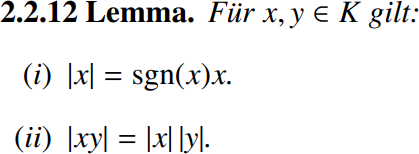
\includegraphics[width = 5 cm]{Kaltenbaeck - Fundament Analysis - Lemma 2-2-12-1.png} \\
      \vspace{0.01 cm}
      \hspace{0.5 cm}
      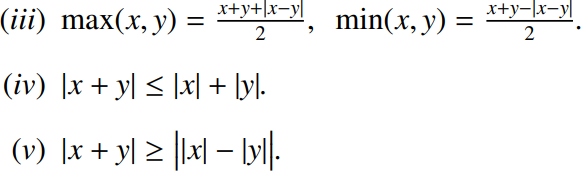
\includegraphics[width = 7 cm]{Kaltenbaeck - Fundament Analysis - Lemma 2-2-12-2.png} \\
      \vspace{0.5 cm}
      \caption{Kaltenbaeck - Fundament Analysis}
      \label{fig:KFAL2.2.12}
    \end{boxedin}
  \end{figure}

  \end{comment}

  Seien $c := 1/2$ und $d := 1$, dann gilt $\ForAlmostAll n \in \N:$

  \begin{multline*}
    c (f(n) + g(n))
    \leq
    \max \Bbraces{f(n), g(n)}
    =
    \frac{f(n) + g(n) + |f(n) - g(n)|}{2} \\
    \leq
    \frac{f(n) + g(n)}{2}
    +
    \frac{f(n) + g(n)}{2}
    =
    d (f(n) + g(n)).
  \end{multline*}

  \item Gegenbeispiel:
  Seien $f \equiv 0$ und $g \equiv 1$, dann gilt $\Forall c, d > 0:$

  \begin{align*}
    c \underbrace{(f(n) + g(n))}_1
    \not \leq
    \underbrace{\min \Bbraces{f(n), g(n)}}_0
    <
    d \underbrace{(f(n) + b(n))}_1.
  \end{align*}

  \begin{align*}
    \implies
    \min \Bbraces{f, g} \not \in \Theta(f + g)
  \end{align*}

  \item Gegenbeispiel:
  Seien $f(n) = n$ und $g(n) = -n$, für $n \in \N$, dann gilt wegen $|f| = |g|$ zwar $f \in \Landau(g)$, aber

  \begin{align*}
    \limsup_{n \to \infty}
    \vbraces
    {
      \frac
      {
        2^{f(n)}
      }{
        2^{g(n)}
      }
    }
    =
    \limsup_{n \to \infty}
    \vbraces
    {
      \frac
      {
        2^{n}
      }{
        2^{-n}
      }
    }
    =
    \limsup_{n \to \infty}
    2^{2n}
    =
    \infty
    \iff
    f \not \in \Landau(g).
  \end{align*}

  Gegenbeispiel:
  Seien $f = \log_2$ und $g = \log_4$, für $n \in \N$, dann gilt wegen $|f| = \log_2{4} |g|$ zwar $f \in \Landau(g)$, aber

  \begin{multline*}
    \limsup_{n  \to \infty}
    \vbraces
    {
      \frac
      {
        2^{f(n)}
      }{
        2^{g(n)}
      }
    }
    =
    \limsup_{n  \to \infty}
    \vbraces
    {
      \frac
      {
        2^{\log_2(n)}
      }{
        2^{\log_4(n)}
      }
    }
    =
    \limsup_{n  \to \infty}
    \vbraces
    {
      \frac
      {
        n
      }{
        2^\frac
        {
          \log_2(n)
        }{
          \log_2(4)
        }
      }
    }
    =
    \limsup_{n  \to \infty}
    \vbraces
    {
      \frac
      {
        n
      }{
        (2^{\log_2(n)})^{1/2}
      }
    } \\
    =
    \limsup_{n  \to \infty}
    \vbraces
    {
      \frac
      {
        n
      }{
        \sqrt{n}
      }
    }
    =
    \limsup_{n  \to \infty}
    \sqrt{n}
    =
    \infty
  \end{multline*}

  \item Gegenbeispiel:
  Sei $f(n) = 1/n$.

  \begin{align*}
    \implies
    \limsup_{n \to \infty}
    \vbraces
    {
      \frac{f(n)}{f(n)^2}
    }
    =
    \limsup_{n \to \infty}
    \vbraces
    {
      \frac{1/n)}{1/n^2}
    }
    =
    \limsup_{n \to \infty} |n|
    =
    \infty
    \iff
    f \not \in \Landau(f^2)
  \end{align*}

  \item Beispiel:

  \begin{align*}
    f(n)
    :=
    \begin{cases}
      0,   & n \in 2 \N, \\
      n^2, & n \in 2 \N - 1,
    \end{cases}
  \end{align*}

  \begin{align*}
    \implies
    \liminf_{n \to \infty}
    \vbraces
    {
      \frac{f(n)}{n}
    }
    & =
    \sup_{n \in \N}
    \inf_{k \geq n}
    \vbraces
    {
      \frac{f(k)}{k}
    }
    =
    0
    \iff
    f(n) \neq \Omega(n), \\
    \limsup_{n \to \infty}
    \vbraces
    {
      \frac{f(n)}{n}
    }
    & =
    \inf_{n \in \N}
    \sup_{k \geq n}
    \vbraces
    {
      \frac{f(k)}{k}
    }
    =
    \infty
    \iff
    f(n) \neq \Landau(n).
  \end{align*}

\end{enumerate}

\end{solution}

% --------------------------------------------------------------------------------


--------------------------------------------------------------------------------

% --------------------------------------------------------------------------------

\begin{exercise}

Zeigen Sie:

\begin{align*}
  f(n) := 2^{2^{\floorbraces{\log_2{(\log_2{n})}}}} = \Landau(n)
\end{align*}

und bestimmen Sie die größte Zahl $c > 0$, sodass

\begin{align*}
  2^{2^{\floorbraces{\log_2{(\log_2{n})}}}} = \Omega(n^c)
\end{align*}

\end{exercise}

% --------------------------------------------------------------------------------

\begin{solution}

\phantom{}

\begin{enumerate}

  \item

  \begin{align*}
    \implies
    \Forall n \in \N:
    2^{2^{\floorbraces{\log_2{(\log_2{n})}}}}
    \leq
    2^{2^{\log_2{(\log_2{n})}}}
    =
    2^{(\log_2{n})}
    =
    n
    =
    \Landau(n)
  \end{align*}

  \item Wir behaupten, dass
  
  \begin{align*}
    1/2 = c := \sup{C},
    \quad
    C := \Bbraces{d > 0: 2^{2^{\floorbraces{\log_2{(\log_2{n})}}}} = \Omega(n^d)}.
  \end{align*}

  \begin{itemize}

    \item
    [\enquote{$\leq$}:]

    \begin{align*}
      & \implies
      \Forall n \in \N:
      2^{2^{\floorbraces{\log_2{(\log_2{n})}}}}
      \geq
      2^{2^{\log_2{(\log_2{n})} - 1}}
      =
      2^{2^{\log_2{(\log_2{(n)})}} / 2}
      =
      (2^{\log_2{n}})^{1/2}
      =
      \sqrt{n}
      =
      \Omega(n^{1/2}) \\
      & \implies
      1/2 \in C
    \end{align*}

    \item
    [\enquote{$\geq$}:]
    Sei $d > 1/2$, dann ist $1/2 - d < 0$.
    Betrachte die Folge $a_n := 2^{2^n} - 1$.

    \begin{align*}
      & \implies
      f(a_n) = 2^{2^{\floorbraces{\log_2{(\log_2{(a_n)})}}}}
      =
      \underbrace
      {
        2^{2^{\floorbraces{\log_2 \pbraces{\log_2 \pbraces{2^{2^n} - 1}}}}}
      }_{
        \stackrel{\text{scharf}}{<}
        2^{2^{\floorbraces{\log_2{\log_2{2^{2^n}}}}}}
        =
        2^{2^n}
      }
      =
      2^{2^{n-1}} \\
      & \implies
      \frac{f(a_n)}{a_n^d}
      =
      \frac{2^{2^{n-1}}}{(2^{2^n} - 1)^d}
      =
      \frac{(2^{2^n})^{1/2}}{(2^{2^n} - 1)^d}
      \leq
      \frac{(2^{2^n})^{1/2}}{(2^{2^n}/2)^d}
      \leq
      2^d \frac{(2^{2^n})^{1/2}}{(2^{2^n})^d}
      =
      2^d (2^{2^n})^{1/2 - d}
      \xrightarrow{n \to \infty}
      0 \\
      & \implies
      \liminf_{n \to \infty}
      \frac{f(n)}{n^d} = 0
      \iff
      f(n) \neq \Omega(n^d) \\
      & \implies
      d \not \in C
    \end{align*}

  \end{itemize}

\end{enumerate}

\end{solution}

% --------------------------------------------------------------------------------


--------------------------------------------------------------------------------

% -------------------------------------------------------------------------------- %

\begin{exercise}[48]

Seien $A = \Bbraces{a_1, \dots, a_n}$ und $B = \Bbraces{b_1, \dots, b_k}$ endliche Mengen.
Sei $P = \Bbraces{p_{i, j} \mid 1 \leq i \leq n, 1 \leq j \leq k}$ eine Menge aussagenlogischer Variablen.
Jede Belegung $b$ von $P$ induziert eine Relation $R_b \subseteq A \times B$ durch $(a_i, b_j) \in R_b$ gdw $b(p_{i, j}) = 1$.
Finden Sie aussagenlogische Formeln $\varphi_1, \varphi_2, \varphi_3, \varphi_4$ so dass:

\begin{enumerate}[label = \arabic*.]
    \item $\hat{b}(\varphi_1) = 1$ gdw $R_b$ ist eine Funktion
    \item $\hat{b}(\varphi_2) = 1$ gdw $R_b$ ist eine injektive Funktion
    \item $\hat{b}(\varphi_3) = 1$ gdw $R_b$ ist eine surjektive Funktion
    \item $\hat{b}(\varphi_4) = 1$ gdw $R_b$ ist eine bijektive Funktion
\end{enumerate}

Für welche $(n, k) \in \N \times \N$ ist $\varphi_2$ unerfüllbar? \\

(
    Anmerkung:
    Die Größe der Formeln hängt von $n$ und $k$ ab.
)

\end{exercise}

% -------------------------------------------------------------------------------- %

\begin{solution}

Nachdem wir Formeln angeben müssen, ist es sicher keine schlechte Idee, die Angabe auch in Formeln aufzuschreiben.

\begin{align*}
  P =
  \begin{Bmatrix}
    p_{11}, & \cdots & p_{1k}, \\
    \vdots  & \ddots & \vdots \\
    p_{n1}, & \cdots & p_{nk}
  \end{Bmatrix},
  \quad
  \begin{matrix}
    A = \Bbraces{a_1, \dots, a_n}, \\
    B = \Bbraces{b_1, \dots, b_k}
  \end{matrix}
\end{align*}

\begin{align*}
  b: p \to \Bbraces{0, 1}
  \rightsquigarrow
  R_b
  =
  \Bbraces
  {
    (a_i, b_j) \in A \times B:
    \:
    \begin{matrix}
      i = 1, \dots, n, \\
      j = 1, \dots, k,
    \end{matrix}
    \quad
    b(p_{ij}) = 1
  }
\end{align*}

\begin{enumerate}[label = \arabic*.]

  \item

  \begin{align*}
    R_b ~\text{Funktion}
    :\iff
    & \Forall a_i \in A:
    \ExistsOnlyOne b_j \in B:
    (a_i, b_j) \in R_b \\
    \iff
    & \Forall a_i \in A:
    \Exists b_j \in B:
    (a_i, b_j) \in R_b
    ~ \land \\
    & \Forall a_i \in A:
    \Forall b_{j_1}, b_{j_2} \in B:
    (a_i, b_{j_1}), (a_i, b_{j_2}) \in R_b
    \implies
    b_{j_1} = b_{j_2} \\
    \iff
    & \Forall a_i \in A:
    \Exists b_j \in B:
    (a_i, b_j) \in R_b
    ~ \land \\
    & \Forall a_i \in A:
    \Forall b_{j_1} \in B:
    (a_i, b_{j_1}) \in R_b
    \implies
    \Forall b_{j_2} \in B \setminus \Bbraces{b_{j_1}}:
    (a_i, b_{j_2}) \not \in R_b
  \end{align*}

  Wir brauchen für unsere Formel also $2$ Bauteile.

  \begin{align*}
    \phi_1
    & :=
    \bigwedge_{i=1}^n \bigvee_{j=1}^kp_{i,j} \\
    \phi_2
    & :=
    \bigwedge_{i=1}^n \bigwedge_{j_1=1}^kp_{i,j_1}
    \to
    \bigwedge_{\substack{j_2=1 \\ j_2\neq j_1}}^{k}\neg p_{i,j_2}
  \end{align*}

  \begin{align*}
    \rightsquigarrow
    \varphi_1 := \phi_1 \land \phi_2
  \end{align*}

  \item Sei $R_b$ eine Funktion.

  \begin{align*}
    R_b ~\text{injektiv}
    :\iff
    & \Forall a_{i_1}, a_{i_2} \in A:
    \Forall b_j \in B:
    (a_{i_1}, b_j), (a_{i_1}, b_j) \in R_b
    \implies
    a_{i_1} = a_{i_2} \\
    \iff
    & \Forall b_j \in B:
    \Forall a_{i_1} \in A:
    (a_{i_1}, b_j) \in R_b
    \implies
    \Forall a_{i_2} \in A \setminus \Bbraces{a_{i_1}}:
    (a_{i_2}, b_j) \not \in R_b
  \end{align*}

  Wir brauchen also noch folgendes, zu $\phi_2$ analoges, Bauteil.

  \begin{align*}
    \phi_3
    :=
    \bigwedge_{j=1}^k \bigwedge_{i_1=1}^np_{i_1,j}
    \to
    \bigwedge_{\substack{i_2=1 \\ i_2\neq i_1}}^{n}\neg p_{i_2,j}
  \end{align*}

  \begin{align*}
    \rightsquigarrow
    \varphi_2
    :=
    \varphi_1 \land \phi_3
  \end{align*}

  % $\varphi_2 = \bigwedge_{i=1}^n \bigvee_{j=1}^k\left(p_{i,j} \land \bigwedge_{l=1,l\neq j}^{k}\neg p_{i,l}\right)
  % \land  \left(\bigwedge_{j=1}^k \bigvee_{i=1}^n\left(p_{i,j} \land \bigwedge_{l=1,l\neq j}^{n}\neg p_{l,j}\right)\right)$

  \item Sei $R_b$ eine Funktion.

  \begin{align*}
    R_b ~\text{surjektiv}
    :\iff
    & \Forall b_j \in B:
    \Exists a_i \in A:
    (a_i, b_j) \in R_b
  \end{align*}

  Wir brauchen also noch folgendes, zu $\phi_1$ analoges, Bauteil.

  \begin{align*}
    \phi_4
    :=
    \bigwedge_{j=1}^k \bigvee_{i=1}^np_{i,j}
  \end{align*}

  \begin{align*}
    \rightsquigarrow
    \varphi_3
    :=
    \varphi_1 \land \phi_4
  \end{align*}

  % $\varphi_3 = \bigwedge_{i=1}^n \bigvee_{j=1}^k\left(p_{i,j} \land \bigwedge_{l=1,l\neq j}^{k}\neg p_{i,l}\right) \land
  % \left(\bigwedge_{j=1}^k \bigvee_{i=1}^np_{i,j}\right)$

  \item Sei $R_b$ eine Funktion.

  \begin{align*}
    R_b ~\text{bijektiv}
    :\iff
    R_b ~\text{injektiv}
    \land
    R_b ~\text{surjektiv}
  \end{align*}

  \begin{align*}
    \rightsquigarrow
    \varphi_4
    :=
    \varphi_2 \land \varphi_3
    =
    \varphi_1 \land \phi_3 \land \phi_4
    =
    \phi_1 \land \phi_2 \land \phi_3 \land \phi_4
  \end{align*}

  % $\varphi_4 = \bigwedge_{i=1}^n \bigvee_{j=1}^k\left(p_{i,j} \land \bigwedge_{l=1,l\neq j}^{k}\neg p_{i,l}\right)
  % \land  \left(\bigwedge_{j=1}^k \bigvee_{i=1}^n\left(p_{i,j} \land \bigwedge_{l=1,l\neq j}^{n}\neg p_{l,j}\right)\right) \land
  % \left(\bigwedge_{j=1}^k \bigvee_{i=1}^np_{i,j}\right)$
\end{enumerate}

Für $k < n$ gibt es keine injektive Funktion von $A$ nach $B$, also ist $\varphi_2$ unerfüllbar, für $k \geq n$ gibt es schon eine, also ist $\varphi_2$ dann erfüllbar.
Das kann man sich auf anschaulich mit einem klassischen Funktions-Diagramm skizzieren:
Zwei getrennte Kreise (Ellipsen), die Punkte beinhalten, die jeweils zwischen den Kreisen verbunden sind.

\end{solution}

% -------------------------------------------------------------------------------- %

\begin{solution}

\phantom{}

\begin{enumerate}[label = \arabic*.]

  \item $\varphi_1 = \bigwedge_{i=1}^n \bigvee_{j=1}^k\left(p_{i,j} \land \bigwedge_{l=1,l\neq j}^{k}\neg p_{i,l}\right)$

  \item $\varphi_2 = \bigwedge_{i=1}^n \bigvee_{j=1}^k\left(p_{i,j} \land \bigwedge_{l=1,l\neq j}^{k}\neg p_{i,l}\right)
  \land  \left(\bigwedge_{j=1}^k \pbraces{\pbraces{\bigvee_{i=1}^n p_{i,j}} \rightarrow \pbraces{\bigvee_{i=1}^n\left(p_{i,j} \land \bigwedge_{l=1,l\neq j}^{n}\neg p_{l,j}\right)}}\right)$

  \item $\varphi_3 = \bigwedge_{i=1}^n \bigvee_{j=1}^k\left(p_{i,j} \land \bigwedge_{l=1,l\neq j}^{k}\neg p_{i,l}\right) \land
  \left(\bigwedge_{j=1}^k \bigvee_{i=1}^np_{i,j}\right)$

  \item $\varphi_4 = \bigwedge_{i=1}^n \bigvee_{j=1}^k\left(p_{i,j} \land \bigwedge_{l=1,l\neq j}^{k}\neg p_{i,l}\right)
  \land  \left(\bigwedge_{j=1}^k \bigvee_{i=1}^n\left(p_{i,j} \land \bigwedge_{l=1,l\neq j}^{n}\neg p_{l,j}\right)\right)$

\end{enumerate}

\end{solution}

% -------------------------------------------------------------------------------- %


--------------------------------------------------------------------------------

\begin{exercise}

Gegeben ist die Funktion $F: \R \to \R:$

\begin{align*}
  F(x) =
  \begin{cases}
    0   & \text{wenn} \enspace x < 0, \\
    1   & \text{wenn} \enspace 0 \leq x < 1, \\
    x^2 & \text{wenn} \enspace 1 \leq x < 2, \\
    5   & \text{wenn} \enspace x \geq 2.
  \end{cases}
\end{align*}

\begin{itemize}
  \item[(a)] Zeigen Sie, dass $F$ eine Verteilungsfunktion ist.
  \item[(b)] Bestimmen Sie $\mu_F(]0, 1[)$, $\mu_F([0, 2])$, $\mu_F(\Q)$.
  \item[(c)] Bestimmen Sie $\Int{e^x}{\mu_F(x)}$.
\end{itemize}

\end{exercise}

--------------------------------------------------------------------------------

\begin{solution}

(a)

\begin{itemize}

  \item \Quote{Rechtsstetigkeit}: $F$ ist stückweise stetig und $\Forall x = 0, 1, 2: F \text{ist rechtsstetig bei} \enspace x$.

  \item \Quote{Steigende Monotonie}: $F$ ist stückweise monoton steigend und $\Forall x = 0, 1, 2: F(x - 0) \leq F(x)$.

\end{itemize}

(b)

\begin{itemize}

  \item $\mu_F(]0, 1[) =$
  \begin{align*}
    \mu_F \pbraces{\bigcup_{n \in \N} \left ] 0, 1 - \frac{1}{n} \right ]}
    =
    \lim_{n \in \N} \mu_F \pbraces{\left ] 0, 1 - \frac{1}{n} \right ]}
    =
    \lim_{n \in \N} F \pbraces{1 - \frac{1}{n}} - F(0)
    = 1 - 1 = 0
  \end{align*}

  \item $\mu_F([0, 2]) =$
  \begin{align*}
    \mu_F \pbraces{\bigcap_{n \in \N} \left ] 0 - \frac{1}{n}, 2 \right ]}
    =
    \lim_{n \in \N} \mu_F \pbraces{\left ] 0 - \frac{1}{n}, 2 \right ]}
    =
    \lim_{n \in \N} F(2) - F \pbraces{0 - \frac{1}{n}}
    =
    5 - 0 = 5
  \end{align*}

  \item $\mu_F(\Q) =$
  \begin{align*}
    \mu_F \pbraces{\sum_{q \in \Q} \Bbraces{q}}
    & =
    \sum_{q \in \Q} \mu_F \pbraces
    {\bigcap_{n \in \N} \left ] q - \frac{1}{n}, q \right ]} \\
    & =
    \sum_{q \in \Q} \lim_{n \in \N} \mu_F \pbraces
    {\left ] q - \frac{1}{n}, q \right ]} \\
    & =
    \sum_{q \in \Q} F(q - 0) - F(q) \\
    & =
    \sum_{x = 0, 1, 2} (F(x) - F(x - 0)) \\
    & =
    (1 - 0) + (1 - 1) + (5 - 4) = 2
  \end{align*}

\end{itemize}

(c) Seien $f = \exp$ und $a_1, \ldots, a_n$ die Sprünge von $F$, sowie $a_0 = - \infty$ und $a_{n+1} = \infty$.

\begin{align*}
  \Int{f}{\mu_F}
  =
  \sum_{i=1}^{n+1} \Int[a_{i-1}][a_i]{f(x) F^\prime(x)}{x} +
  \sum_{i=1}^n f(a_i) (F(a_i) - F(a_i - 0))
\end{align*}

Also ...

\begin{align*}
  \Int{e^x}{\mu_F(x)}
  & =
  \underbrace{\Int[-\infty][0]{e^x 0}{x}}_0
  +
  \underbrace{\Int[0][1]{e^x 0}{x}}_0
  +
  \Int[1][2]{e^x 2x}{x}
  +
  \underbrace{\Int[2][\infty]{e^x 0}{x}}_0 \\
  & +
  e^0 \underbrace{(F(0) - F(0 - 0))}_{= 1-0 = 1}
  +
  e^1 \underbrace{(F(1) - F(1 - 0))}_{= 1-1 = 0}
  +
  e^2 \underbrace{(F(2) - F(2 - 0))}_{= 5-4 = 1} \\
  & =
  e^x 2x |_1^2 - 2 \Int[1][2]{e^x}{x} + 1 + e^2 \\
  & =
  (4e^2 - 2e) - 2 (e^2 - e) + 1 + e^2
  =
  1 + 3e^2
\end{align*}

\end{solution}


--------------------------------------------------------------------------------

% --------------------------------------------------------------------------------

\begin{exercise}[Exercise 3.8]

Suppose $\gamma = 0.5$ and the following sequence of rewards is received $R_1 = -1$, $R_2 = 2$, $R_3 = 6$, $R_4 = 3$, and $R_5 = 2$, with $T = 5$.
What are $G_0, G_1 , \dots, G_5$?
Hint:
Work backwards.    

\end{exercise}

% --------------------------------------------------------------------------------

\begin{solution}

ToDo!

\end{solution}

% --------------------------------------------------------------------------------


--------------------------------------------------------------------------------

\setcounter{exercise}{0}

\section{Messbare Funktionen}

--------------------------------------------------------------------------------

\begin{exercise}

Es sei $\Omega = \N$, $\mathfrak{S} = 2^\N$, $\mu(A) = \sum_{x \in A} 2^{-x}$. Wann konvergiert die Funktionenfolge $f_n$ im Maßraum $(\Omega, \mathfrak{S}, \mu)$

\begin{itemize}
  \item[(a)] fast überall
  \item[(b)] fast gleichmäßig
  \item[(c)] im Maß?
\end{itemize}

\end{exercise}

\begin{solution}

(a) $f_n \xrightarrow{\text{f.ü.}} f : \Leftrightarrow$

\begin{align*}
  \Exists N \in \mathfrak{S}:
  \mu(N) = 0,
  f_n|_{N^\complement} \xrightarrow{\text{punktw.}} f|_{N^\complement}
\end{align*}

Aber ...

\begin{align*}
  \mu(N) = 0
  \Leftrightarrow
  \sum_{x \in N} 2^{-x} = 0
  \Leftrightarrow
  N = \emptyset
\end{align*}

Also ...

\begin{align*}
  f_n \xrightarrow{\text{f.ü.}} f
  \Leftrightarrow
  f_n \xrightarrow{\text{punktw.}} f
\end{align*}

\end{solution}

(b) $f_n \xrightarrow{\mu \text{-fast glm.}} f : \Leftrightarrow$

\begin{align*}
  \Forall \epsilon > 0:
  \Exists A_\epsilon \in \mathfrak{S}:
  \mu(A_\epsilon) < \epsilon,
  f_n|_{A_\epsilon^\complement} \xrightarrow{\text{glm.}} f|_{A_\epsilon^\complement}
\end{align*}

$\mu$ ist ein endliches Maß, weil

\begin{align*}
  \mu(\Omega) = \mu(\N) = \sum_{n \in \N} \frac{1}{2^n} = 2 < \infty.
\end{align*}

Laut \Quote{Egorov}, gilt also

\begin{align*}
  f_n \xrightarrow{\mu \text{-fast glm.}} f
  \Leftrightarrow
  f_n \xrightarrow{\text{f.ü.}} f.
\end{align*}

(c) $f_n \xrightarrow{\text{im Maß}} f : \Leftrightarrow$

\begin{align*}
  \Forall \epsilon > 0:
  \lim_{n \to \infty} \mu(|f_n - f| > \epsilon) = 0
\end{align*}

zz: $f_n \xrightarrow{\text{im Maß}} f \Leftrightarrow f_n \xrightarrow{\text{punktw.}} f$ \\

Nun gilt

\begin{align*}
  \mu(|f_n - f| > \epsilon)
  =
  \sum_{x \in [|f_n - f| > \epsilon]} 2^{-x}
\end{align*}

\begin{itemize}

  \item[\Quote{$\Rightarrow$}:] Angenommen,
  \begin{align*}
    \Exists x \in \Omega:
    \Exists \epsilon > 0:
    \Forall N \in \N:
    \Exists n \geq N:
    |f_n(x) - f(x)| > \epsilon,
  \end{align*}
  dann muss $[|f_n - f| > \epsilon] \neq \emptyset$, also $\mu(|f_n - f| > \epsilon) \neq 0$ und somit $\lim_{n \to \infty} \mu(|f_n - f| > \epsilon) \neq 0$.

  \item[\Quote{$\Leftarrow$}:] Angenommen,
  \begin{align*}
    \Exists \epsilon > 0:
    \Forall N \in \N:
    \Exists n \leq N:
    \mu(|f_n - f| > \epsilon) \neq 0,
  \end{align*}
  dann muss $[|f_n - f| > \epsilon] \neq 0$, also $\Exists x \in \Omega: |f_n - f| > \epsilon$.

\end{itemize}

--------------------------------------------------------------------------------

\begin{exercise}

Es sei $\Omega = \N$, $\mathfrak{S} = 2^\N$, $\mu(A) = |A|$. Wann konvergiert die Funktionenfolge $f_n$ im Maßraum $(\Omega, \mathfrak{S}, \mu)$

\begin{itemize}
  \item[(a)] fast überall
  \item[(b)] fast gleichmäßig
  \item[(c)] im Maß?
\end{itemize}

\end{exercise}

\begin{solution}

Man beachte, dass $\Forall A \in 2^\N: |A| = 0 \Leftarrow A = \emptyset$, d.h. $\emptyset$ ist die einzige Nullmenge. Somit gilt eine Aussage genau dann fast überall, wenn sie auf $\emptyset^\complement = \N$ gilt, also überall.

(a)

\begin{align*}
  f_n \xrightarrow[n \to \infty]{\text{f.ü.}} f
  \Leftarrow
  f_n \xrightarrow[n \to \infty]{\text{punktw.}} f
\end{align*}

(b)

\begin{align*}
  f_n \xrightarrow[n \to \infty]{\text{fast glm.}} f
  \Leftarrow
  f_n \xrightarrow[n \to \infty]{\text{glm.}} f
\end{align*}

(c)

\end{solution}

--------------------------------------------------------------------------------

\begin{exercise}

$f: \R \to \R$ sei überall differenzierbar. Zeigen Sie, dass $f^\prime$ Borel-messbar ist.

\end{exercise}

\begin{solution}

\begin{align*}
  \Forall n \in \N:
  f_n: x \mapsto \frac{f(x + 1/n) - f(x)}{1/n},
  \enspace \text{messb.}
  \Rightarrow
  f^\prime = \lim_{n \to \infty} f_n
  \enspace \text{messb.}
\end{align*}

\end{solution}

--------------------------------------------------------------------------------

\begin{exercise}

\begin{itemize}
  \item[(a)] Definieren Sie: messbare Funktion, Treppenfunktion, Konvergenz im Maß, Konvergenz fast überall, Konvergenz fast gleichmäßig.
  \item[(b)] Formulieren und beweisen Sie den Approximationssatz für reellwertige messbare Funktionen.
\end{itemize}

\end{exercise}

\begin{solution}

(a) $f: (\Omega_1, \mathfrak{S}_1) \to (\Omega_2, \mathfrak{S}_2) \enspace \text{Treppenfunktion}
: \Leftrightarrow
\Exists a_1, \ldots, a_n \in \Omega_2,
\Exists A_1, \ldots, A_n \in \mathfrak{S}_1:$

\begin{align*}
  \sum_{i=1}^n A_i = \Omega_1, \enspace
  \sum_{i=1}^n a_i A_i = f
\end{align*}

Rest siehe Aufgabe 1 und 12 (a).

(b) Siehe Skript.

\end{solution}

--------------------------------------------------------------------------------

\begin{exercise}

Hier könnte Ihre Werbung stehen!

\begin{itemize}
  \item Definieren Sie: messbare Funktion, Treppenfunktion, Konvergenz im Maß, Konvergenz fast überall, Konvergenz fast gleichmäßig.
  \item In welchem Sinn (fast überall gleichmäßig/fast gleichmäßig/fast überall/im Maß) konvergieren die folgenden Folgen in $(\R, \mathfrak{B}, \lambda)$?
  \begin{itemize}
    \item[i.] $f_n(x) = \sin(x)/n$
    \item[ii.] $f_n(x) = e^{-n |x|}$
    \item[iii.] $f_n(x) = x/n$
    \item[iv.] $f_n(x) = f_n(x) =
    \begin{cases}
      1 & \text{wenn} \enspace \sqrt{n} - \floor{\sqrt{n}} \leq x \leq \sqrt{n+1} - \floor{\sqrt{n}} \\
      0 & \text{sonst}.
    \end{cases}$
  \end{itemize}
\end{itemize}

\end{exercise}

\begin{solution}

(a) Siehe Aufgabe 7 (a) \\

(b) Hier könnte Ihre Werbung stehen!

\begin{itemize}

  \item[i.]
  \begin{align*}
     \norm[\infty]{f_n}
     =
     \sup_{x \in \R} \vbraces{\sin(x)/n}
     =
     1/n
     \xrightarrow[n \to \infty]{} 0 \\
     \Rightarrow
     f_n \xrightarrow[n \to \infty]{\text{glm.}} 0
     \Rightarrow
     f_n \xrightarrow[n \to \infty]{\text{fast glm.}} 0
     \Rightarrow
     f_n \xrightarrow[n \to \infty]{\text{f.ü.}} 0,
     \enspace
     f_n \xrightarrow[n \to \infty]{\text{im Maß}} 0
   \end{align*}

  \item[ii.]
  \begin{align*}
    \Forall A \subseteq \R \setminus \Bbraces{0}:
    \norm[\infty]{f_n|_A}
    =
    \sup_{x \in A} \vbraces{e^{-n |x|}}
    =
    e^{-n \inf_{x \in A} |x|}
    \xrightarrow[n \to \infty]{} 0 \\
    \Rightarrow
    f_n \xrightarrow[n \to \infty]{\text{fast glm.}} 0
    \Rightarrow
    f_n \xrightarrow[n \to \infty]{\text{f.ü.}} 0,
    \enspace
    f_n \xrightarrow[n \to \infty]{\text{im Maß}} 0
  \end{align*}
  Sei $N \in \mathfrak{B}$, mit $\lambda(N) = 0$, dann gilt trotzdem noch $\Forall \epsilon > 0: \vbraces{B(0, \epsilon) \cap N^\complement} = \infty$, also konvergiert $(f_n)$ nicht fast überall gleichmäßig.

  \item[iii.]
  \begin{align*}
    f_n \xrightarrow[n \to \infty]{\text{punktw.}} 0
    \Rightarrow
    f_n \xrightarrow[n \to \infty]{\text{f.ü.}} 0
  \end{align*}
  $\Forall \epsilon > 0, \Forall n \in \N:$
  \begin{align*}
    \lambda(x/n > \epsilon)
    =
    \lambda(x > \epsilon n)
    =
    \lambda(]\epsilon n, \infty])
    =
    \infty
  \end{align*}
  Also konvergiert $(f_n)$ nicht im Maß. \\
  Wenn $(f_n)$ fast (überall) gleichmäßig konvergiert, dann offensichtlich gegen $0$. Aber $\Forall \epsilon > 0, \Forall N \in \mathfrak{B}:$
  \begin{align*}
    \lambda(N) < \epsilon
    \Rightarrow
    \Forall n \in \N:
    \norm[\infty]{f_n|_{N^\complement}}
    =
    \sup_{x \in N^\complement} |x|/n
    =
    \infty
  \end{align*}
  Also konvergiert $(f_n)$ weder fast gleichmäßig, noch fast überall gleichmäßig. \\

  \item[iv.] $\Forall \epsilon > 0:$
  \begin{align*}
    \lambda(|f_n| > \epsilon)
    =
    \lambda(f_n = 1)
    =
    \lambda
    ([\sqrt{n} - \floor{\sqrt{n}}, \sqrt{n+1} - \floor{\sqrt{n}}])
    =
    \sqrt{n+1} - \sqrt{n}
    \xrightarrow[n \to \infty]{} 0 \\
    \Rightarrow
    f_n \xrightarrow[n \to \infty]{\text{im Maß}} 0
  \end{align*}
  $\Forall q \in \N^2:$
  \begin{align*}
    ]0, 1]
    =
    \sum_{i = q}^{(\sqrt{q}+1)^2-1}
    \left ]
    \sqrt{i} - \floor{\sqrt{i}}, \sqrt{i+1} - \floor{\sqrt{i}}
    \right ]
  \end{align*}
  Also, muss $\Forall x \in \: ]0, 1], \Forall N \in \N: \Exists n, m \geq N:$
  \begin{align*}
    |f_n(x) - f_m(x)| = 1,
  \end{align*}
  und es konvergiert $(f_n)$ nicht fast überall und somit auch weder fast gleichmäßig, noch fast überall gleichmäßig.

\end{itemize}

\end{solution}

--------------------------------------------------------------------------------

\begin{exercise}

Hier könnte Ihre Werbung stehen!

\begin{itemize}
  \item Definieren Sie: messbare Funktion, Treppenfunktion, Konvergenz im Maß, Konvergenz fast überall, Konvergenz fast gleichmäßig.
  \item In welchem Sinn (fast überall gleichmäßig/fast gleichmäßig/fast überall/im Maß) konvergieren die folgenden Folgen in $(\R, \mathfrak{B}, \lambda)$?
  \begin{itemize}
    \item[i.] $f_n(x) = \sin(x)/n$
    \item[ii.] $f_n(x) = e^{-n |x|}$
    \item[iii.] $f_n(x) = x/n$
    \item[iv.] $f_n(x) = f_n(x) =
    \begin{cases}
      1 & \text{wenn} \enspace \sqrt{n} - \floor{\sqrt{n}} \leq x \leq \sqrt{n+1} - \floor{\sqrt{n}} \\
      0 & \text{sonst}.
    \end{cases}$
  \end{itemize}
\end{itemize}

\end{exercise}

\begin{solution}

Siehe Aufgabe 8.

\end{solution}

--------------------------------------------------------------------------------

\begin{exercise}

Hier könnte Ihre Werbung stehen!

\begin{itemize}
  \item[(a)] Definieren Sie: messbare Funktion, Treppenfunktion, Konvergenz im Maß, Konvergenz fast überall, Konvergenz fast gleichmäßig.
  \item[(b)] $f_n$, $n \in \N$ und $f$ seien reellwertige messbare Funktionen auf dem Maßraum $(\Omega, \mathfrak{S}, \mu)$. Zeigen Sie:
  \begin{itemize}
    \item[i.] Wenn $f_n \to f$ fast überall und $g: \R \to \R$ stetig ist, dann $g \circ f_n \to g \circ f$ fast überall.
    \item[ii.] Wenn $f_n \to f$ im Maß und $g: \R \to \R$ gleichmäßig stetig ist, dann $g \circ f_n \to g \circ f$ im Maß.
    \item[iii.] Geben Sie ein Beispiel einer Folge $f_n$ und einer stetigen Funktion $g$, sodass $f_n$ im Maß konvergiert, aber nicht $g \circ f_n$.
  \end{itemize}
\end{itemize}

\end{exercise}

\begin{solution}

(a) Siehe Aufgabe 1 (a) und Kapitel 4 Aufgabe 7 (a). \\

(b) i. Wegen der Konvergenz fast überall von $(f_n)$, gilt

\begin{align*}
  \Exists N \in \mathfrak{S}:
  \mu(N) = 0,
  \Forall \omega \in N^\complement:
  \Forall \delta > 0:
  \Exists n_0 \in \N:
  \Forall n \geq n_0:
  |f_n(\omega) - f(\omega)| < \delta.
\end{align*}

Wegen der Stetigkeit von $g$, gilt

\begin{align*}
  \Forall x \in \R:
  \Exists \delta > 0:
  \Forall y \in \R:
  |x - y| < \delta
  \Rightarrow
  |g(x) - g(y)| < \epsilon.
\end{align*}

Damit folgt die Konvergenz fast überall von $(g \circ f_n)$ ...

\begin{align*}
  \Forall \omega \in N^\complement:
  \Forall \epsilon > 0:
  \Exists n_0^\prime \in \N:
  \Forall n \geq n_0^\prime:
  |g(f_n(\omega)) - g(f(\omega))| < \epsilon
\end{align*}

ii. Wegen der Konvergenz im Maß von $(f_n)$, gilt

\begin{align*}
  \Forall \delta > 0:
  \mu(|f_n - f| > \delta)
  \xrightarrow[n \to \infty]{} 0.
\end{align*}

Wegen der gleichmäßigen Stetigkeit von $g$, gilt

\begin{align*}
  \Forall \epsilon > 0:
  \Exists \delta > 0:
  \Forall x, y \in \R:
  |x - y| \leq \delta
  \Rightarrow
  |g(x) - g(y)| \leq \epsilon
\end{align*}

Damit folgt die Konvergenz im Maß von $(g \circ f_n)$ ...

\begin{align*}
  \Forall \epsilon > 0:
  \mu(|g \circ f_n - g \circ f| > \epsilon)
  \leq
  \mu(|f_n - f| > \delta)
  \xrightarrow[n \to \infty]{} 0
\end{align*}

\end{solution}

--------------------------------------------------------------------------------

\begin{exercise}

Hier könnte Ihre Werbung stehen!

\begin{itemize}
  \item[(a)] Definieren Sie: Konvergenz fast überall, fast überall gleichmäßig, fast gleichmäßig, im Maß.
  \item[(b)]  Gegeben ist der Maßraum $(\N, 2^\N, \mu)$ mit $\mu(\Bbraces{x}) = 2^{-x}$, $x \in \N$. Zeigen Sie, dass in diesem Maßraum die Konvergenzen fast überall, fast gleichmäßig und im Maß äquivalent sind.
\end{itemize}

\end{exercise}

\begin{solution}

(a) Siehe Aufgabe 1. \\

(b) Hier könnte Ihre Werbung stehen!

\begin{itemize}

  \item \Quote{f.ü. $\Rightarrow$ fast glm.}: $\mu$ ist ein endliches Maß, weil
  \begin{align*}
    \mu(\N)
    =
    \sum_{x \in \N} \mu(\Bbraces{x})
    =
    \sum_{x \in \N} 2^{-x}
    =
    2 < \infty.
  \end{align*}
  Also gilt, laut \Quote{Egorov},
  \begin{align*}
    f_n \xrightarrow[n \to \infty]{\text{f.ü.}} f
    \Rightarrow
    f_n \xrightarrow[n \to \infty]{\text{fast glm.}} f.
  \end{align*}

  \item \Quote{fast glm. $\Rightarrow$ im Maß}: Zudem, gilt immer
  \begin{align*}
    f_n \xrightarrow[n \to \infty]{\text{fast glm.}} f
    \Rightarrow
    f_n \xrightarrow[n \to \infty]{\text{im Maß}} f.
  \end{align*}

  \item \Quote{im Maß $\Rightarrow$ f.ü.}:
  \begin{align*}
    f_n \xrightarrow[n \to \infty]{\text{im Maß}} f
  \end{align*}
  heißt, dass $\Forall \epsilon > 0:$
  \begin{align*}
    \sum_{x \in [|f_n - f| > \epsilon]} 2^{-x}
    =
    \mu(|f_n - f| > \epsilon)
    \xrightarrow[n \to \infty]{} 0,
  \end{align*}
  also gilt $\Forall x \in \N: \Exists N \in \N: \Forall n \geq N:$
  \begin{align*}
    x \notin [|f_n - f| > \epsilon]
    \Leftrightarrow
    |f_n(x) - f(x)| \leq \epsilon,
  \end{align*}
  und somit schließlich
  \begin{align*}
    f_n \xrightarrow[n \to \infty]{\text{f.ü.}} f.
  \end{align*}

\end{itemize}

\end{solution}

--------------------------------------------------------------------------------

\begin{exercise}

Hier könnte Ihre Werbung stehen!

\begin{itemize}
  \item[(a)] Definieren Sie messbare Funktion, maßtreue Funktion.
  \item[(b)] Auf $\Omega = \N$ ist die Funktion
  \begin{align*}
    f(x) = x^2 - 3x
  \end{align*}
  gegeben. Bestimmen Sie die kleinste Sigmaalgebra $\mathfrak{S}$ über $\Omega$, für die $f$ $\mathfrak{S}$-messbar ist.
\end{itemize}

\end{exercise}

\begin{solution}

(a) Hier könnte Ihre Werbung stehen!

\begin{itemize}

  \item $f: (\Omega_1, \mathfrak{S}_1) \to (\Omega_2, \mathfrak{S}_2) : \Leftrightarrow f^{-1}(\mathfrak{S}_2) \subseteq \mathfrak{S}_1$

  \item $f: (\Omega_1, \mathfrak{S}_1, \mu_1) \to (\Omega_2, \mathfrak{S}_2, \mu_2) \enspace \text{maßtreu} : \Leftrightarrow \mu_1 \circ f^{-1} = \mu_2$

\end{itemize}

(b) Das wäre dann die initiale Sigmaalgebra

\begin{align*}
  \mathfrak{S}
  =
  f^{-1}(\mathfrak{B})
  =
  \Bbraces{\Bbraces{n \in \N: n^2 - 3n \in A}: A \in \mathfrak{B}}.
\end{align*}

zz: $\mathfrak{S} = \mathfrak{S}^\prime := \Bbraces{B \in 2^\N: 1 \in B \Leftrightarrow 2 \in B}$

\begin{itemize}

  \item[\Quote{$\subseteq$}:] $f$ ist bis auf $1, 2$ injektiv.

  \item[\Quote{$\supseteq$}:] $\Forall x \in \R: \Bbraces{x} \in \mathfrak{B}$

\end{itemize}

\end{solution}

--------------------------------------------------------------------------------

\begin{exercise}

Hier könnte Ihre Werbung stehen!

\begin{itemize}
  \item[(a)] Definieren Sie Konvergenz im Maß, fast überall, fast gleichmäßig, fast überall gleichmäßig.
  \item[(b)] $(X_n)$ sei eine Folge von unabhängigen Zufallsvariablen. Zeigen Sie, dass genau dann fast sicher
  \begin{align*}
    \lim_{n \to \infty} X_n = 0
  \end{align*}
  gilt, wenn für jedes $\epsilon > 0$
  \begin{align*}
    \sum_{n \in \N} \P(|X_n| > \epsilon) < \infty.
  \end{align*}
\end{itemize}

\end{exercise}

\begin{solution}

(a) Siehe Aufgabe 1. \\

(b) Hier könnte Ihre Werbung stehen!

\begin{itemize}

  \item[\Quote{$\Rightarrow$}:] Angenommen, $\Exists \epsilon > 0:$
  \begin{align*}
    \sum_{n \in \N} \P(|X_n| > \epsilon) = \infty,
  \end{align*}
  dann gilt laut dem \Quote{zweiten Lemma von Borel-Cantelli}, dass
  \begin{align*}
    \P(\limsup_{n \in \N} [|X_n| > \epsilon]) = 1.
  \end{align*}
  $\limsup_{n \in \N} [|X_n| > \epsilon]$ ist dabei die Menge aller Punkte, die in unendlich vielen $[|X_n| > \epsilon]$ enthalten ist.

  \item[\Quote{$\Leftarrow$}:]
  $1 - \P(|X_n| \leq \epsilon)
  =
  \P(|X_n| > \epsilon)
  \xrightarrow[n \to \infty]{} 0$

\end{itemize}

\end{solution}

--------------------------------------------------------------------------------

\setcounter{exercise}{0}

\section{Das Integral}

--------------------------------------------------------------------------------

\begin{exercise}

Es sei

\begin{align*}
  F(x) =
  \begin{cases}
    0         & \text{für} \enspace x < 0 \\
    x         & \text{für} \enspace 0 \leq x < 1 \\
    (x + 1)^2 & \text{für} \enspace 1 \leq x \leq 2 \\
    0         & \text{für} \enspace x \geq 2
  \end{cases}
\end{align*}

\begin{itemize}
  \item[(a)] Zeigen Sie: $F$ ist eine Verteilungsfunktion
  \item[(b)] Bestimmen Sie $\Int{f}{\mu_F}$ für $f(x) = x^2$.
\end{itemize}

\end{exercise}

\begin{solution}

(a) Hier könnte Ihre Werbung stehen!

\begin{itemize}

  \item \Quote{Rechtsstetigkeit}: $F$ ist stückweise stetig und $\Forall x = 0, 1, 2: F \text{ist rechtsstetig bei} \enspace x$.

  \item \Quote{Steigende Monotonie}: $F$ ist stückweise monoton steigend und $\Forall x = 0, 1, 2: F(x - 0) \leq F(x)$.

\end{itemize}

(b)

\begin{align*}
  \Int{f}{\mu_F}
  & =
  \Int[-\infty][0]{f(x) \underbrace{F^\prime(x)}_0}
  +
  \Int[0][1]{f(x) \underbrace{F^\prime(x)}_1}
  +
  \Int[1][2]{f(x) \underbrace{F^\prime(x)}_{2 (x+1)}}
  +
  \Int[2][\infty]{f(x) \underbrace{F^\prime(x)}_0} \\
  & +
  f(0) \underbrace{(F(0) - F(0 - 0))}_0
  +
  \underbrace{f(1)}_1 \underbrace{(F(1) - F(1 - 0))}_{= 4-1 = 3}
  +
  \underbrace{f(2)}_4 \underbrace{(F(2) - F(2 - 0))}_{= 9-9 = 0} \\
  & =
  \frac{1}{3}
  +
  2 \underbrace
  {
    \Int[1][2]{x^2 (x + 1)}{x}
  }_{
    = \frac{x^4}{4} |_1^2 + \frac{x^3}{3} |_1^2
    = 4 - \frac{1}{4} + \frac{8}{3} - \frac{1}{3}
  }
  =
  \frac{25}{2}
\end{align*}

\end{solution}

--------------------------------------------------------------------------------

\begin{exercise}

Es sei

\begin{align*}
  F(x) =
  \begin{cases}
                            & \text{wenn} \enspace x < 0, \\
    1 - \frac{1}{2} e^{-x}  & \text{wenn} \enspace x \geq 0.
  \end{cases}
\end{align*}

\begin{itemize}
  \item[(a)] Zeigen Sie: $F$ ist eine Verteilungsfunktion.
  \item[(b)] Bestimmen Sie $\Int{f(x)}{\mu_F(x)}$ für $f(x) = e^{-x}$.
\end{itemize}

\end{exercise}

\begin{solution}

(a) Hier könnte Ihre Werbung stehen!

\begin{itemize}

  \item \Quote{Rechtsstetigkeit}: $F$ ist stückweise stetig und $\Forall x = 0: F \text{ist rechtsstetig bei} \enspace x$.

  \item \Quote{Steigende Monotonie}: $F$ ist stückweise monoton steigend und $\Forall x = 0: F(x - 0) \leq F(x)$.

\end{itemize}

(b)

\begin{align*}
  \Int{f}{\mu_F}
  & =
  \Int[-\infty][0]{f(x) \underbrace{F^\prime(x)}_0}
  +
  \Int[0][\infty]
  {
    \underbrace{f(x)}_{e^{-x}}
    \underbrace{F^\prime(x)}_{\frac{1}{2} e^{-x}}
  }
  +
  \underbrace{f(0)}_1 \underbrace{(F(0) - F(0 - 0))}_\frac{1}{2}
  & =
  \frac{1}{2} \underbrace
  {
    \Int[0][\infty]{e^{-2x}}{x}
  }_{
    = -\frac{1}{2} e^{-2x} |_0^\infty
    = -\frac{1}{2}
  }
  +
  \frac{1}{2}
  =
  -\frac{1}{4} + \frac{1}{2} = \frac{1}{4}
\end{align*}

\end{solution}

--------------------------------------------------------------------------------

\begin{exercise}

Hier könnte Ihre Werbung stehen!

\begin{itemize}
  \item[(a)] Definieren Sie das Integral einer nichtnegativen Treppenfunktion, einer nichtnegativen messbaren Funktion, einer messbaren und einer fast uberall messbaren Funktion.
  \item[(b)] Es sei
  \begin{align*}
    F(x) =
    \begin{cases}
      0     & \text{wenn} \enspace  x < 0, \\
      x + 1 & \text{wenn} \enspace 1 \leq x < 2, \\
      2x^2  & \text{wenn} \enspace 2 \leq x < 3, \\
      20    & \text{wenn} \enspace 3 \leq x.
    \end{cases}
  \end{align*}
  Überzeugen Sie sich, dass $F$ eine Verteilungsfunktion ist und bestimmen Sie $\Int{f}{\mu_F}$ für $f(x) = e^x$.
  \item[(c)] Formulieren und beweisen Sie den Satz von der Konvergenz durch Majorisierung.
\end{itemize}

\end{exercise}

\begin{solution}

(a) Sei $t = \sum_{i=1}^n a_i A_i$ eine nichtnegative, messbare Treppenfunktion auf $(\Omega, \mathfrak{S}, \mu)$, dann

\begin{align*}
  \Int{t}{\mu} := \sum_{i=1}^n a_i \mu(A_i).
\end{align*}

Sei $f$ eine nichtnegative, messbare Funktion, dann

\begin{align*}
  \Int{f}{\mu} := \sup \Bbraces{\Int{t}{\mu}: f \geq t \geq 0, t \text{Treppenf.}}.
\end{align*}

Sei $f$ eine messbare Funktion, dann

\begin{align*}
  \Int{f}{\mu} := \Int{f^+}{\mu} - \Int{f^-}{\mu}.
\end{align*}

Sei $f$ eine fast überall messbare Funktion, d.h. $\Exists N \in \mathfrak{S}: \mu(N) = 0, fN^\complement \enspace \text{messb.}$, dann

\begin{align*}
  \Int{f}{\mu} := \Int[N^\complement]{f}{\mu}.
\end{align*}

\end{solution}

--------------------------------------------------------------------------------

\begin{exercise}

$(X_n)$ sei eine Folge von unabhängigen, auf $[0, 1]$ gleichverteilten Zufallsvariablen. Gegen welchen Wert konvergiert

\begin{align*}
  (\prod_{i=1}^n)^\frac{1}{n}?
\end{align*}

\end{exercise}

\begin{solution}

$\ln$ ist messbar, also auf $(\ln X_n)$ unabhängig.

\begin{align*}
  \lim_{n \to \infty}
  \pbraces{\prod_{i=1}^n X_i}^\frac{1}{n}
  & =
  \lim_{n \to \infty}
  \exp \ln \pbraces{\pbraces{\prod_{i=1}^n X_i}^\frac{1}{n}}
  =
  \lim_{n \to \infty}
  \exp \pbraces{\frac{1}{n} \sum_{i=1}^n \ln X_i} \\
  & =
  \exp \pbraces
  {\lim_{n \to \infty} \frac{1}{n} \sum_{i=1}^n \ln X_i}
  =
  \exp \E(\ln X_1)
  =
  \exp \underbrace{\Int[0][1]{\ln(x) \frac{1}{1-0}}{x}}_{-\infty} = 0
\end{align*}

\end{solution}

--------------------------------------------------------------------------------

\begin{exercise}

$(X_n)$ sei eine Folge von unabhängigen Zufallsvariablen mit $\P(X_n = 1) = \P(X_n = -1) = 1/2$, $(a_n)$ eine Folge von reellen Zahlen. Zeigen Sie, dass die Reihe

\begin{align*}
  \sum_{n \in \N} a_n X_n
\end{align*}

genau dann fast sicher konvergiert, wenn

\begin{align*}
  \sum_{n \in \N} a_n^2 < \infty.
\end{align*}

\end{exercise}

\begin{solution}

Wir benützen den \Quote{Dreireihensatz von Kolmogorov}: Wenn $(X_n)$ unabhängige Zufallsvariablen sind, dann

\begin{align*}
  \sum_{n \in \N} X_n
  \enspace \text{konv. f.s.}
  \Leftrightarrow
  \Forall \epsilon > 0:
  \sum_{n \in \N} \P(|X_n| > \epsilon),
  \sum_{n \in \N} \E(X_n [|X_n| \leq \epsilon]),
  \sum_{n \in \N} \V(X_n [|X_n| \leq \epsilon])
  < \infty.
\end{align*}

Zuerst bemerken wir, dass

\begin{align*}
  1
  =
  \P(X_n = 1) + \P(X_n = -1)
  =
  \P(X_n = \pm 1)
  =
  \P(|X_n| = 1)
  =
  \P(X_n^2 = 1)
  \Rightarrow
  \P(X_n \neq \pm 1) = 0.
\end{align*}

Damit berechnet man die Erwartungswerte

\begin{itemize}

  \item $\E(X_n) = 1 \cdot \P(X_n = 1) + (-1) \cdot \P(X_n = -1) = 0$,

  \item $\E(X_n [|X_n| \leq \epsilon]) \leq \E(X_n) = 0$,

  \item $\E(X_n^2) = 1 \cdot \P(X_n^2 = 1) = 1$,

  \item $\E(X_n^2 [|X_n| \leq \epsilon]) = \E(X_n^2 [X_n^2 \leq \epsilon^2]) =
  \begin{cases}
    \E(X_n^2) = 1 & \text{wenn} \enspace \epsilon^2 \geq 1 \\
    0             & \text{sonst}
  \end{cases}$,

\end{itemize}

und Varianzen (mit dem \Quote{Verschiebungssatz von Steiner})

\begin{itemize}

  \item $\V(X_n) = \E(X_n^2) - \E(X_n)^2 = 1^2 - 0 = 1$

  \item $\V(X_n [X_n \leq \epsilon]) = \E(X_n^2 [X_n \leq \epsilon]) - \E(X_n [X_n \leq \epsilon])^2 =
  \begin{cases}
    \E(X_n^2) = 1 & \text{wenn} \enspace \epsilon^2 \geq 1 \\
    0             & \text{sonst}
  \end{cases}$

\end{itemize}

\begin{itemize}

  \item[\Quote{$\Rightarrow$}] $\Exists \epsilon > 0$
  \begin{align*}
    \infty
    >
    \sum_{n \in \N} \V(a_n X_n [|a_n X_n| \leq \epsilon])
    =
    \sum_{n \in \N} a_n^2
  \end{align*}

  \item[\Quote{$\Leftarrow$}]
  \begin{itemize}

    \item $a_n^2 \to 0
    \Rightarrow
    |a_n| \to 0
    \Rightarrow
    |a_n X_n| \to 0$,
    d.h. $\Forall \epsilon > 0: \Exists N \in \N: \Forall n \geq N: |a_n X_n| < \epsilon$ und
    \begin{align*}
      \sum_{n \in \N} \P(X_n > \epsilon) < \infty.
    \end{align*}

    \item
    \begin{align*}
      \sum_{n \in \N} \E(a_n X_n [|a_n X_n| \leq \epsilon])
      \leq
      \sum_{n \in \N} a_n \E(X_n) = 0
    \end{align*}

    \item
    \begin{align*}
      \sum_{n \in \N} \E(a_n X_n [|a_n X_n| \leq \epsilon])
      \leq
      \sum_{n \in \N} a_n^2 \V(X_n)
      =
      \sum_{n \in \N} a_n^2
    \end{align*}

  \end{itemize}

\end{itemize}

\end{solution}

--------------------------------------------------------------------------------


\end{document}
